\documentclass[11pt, a4paper]{article}
\usepackage[utf8]{inputenc}
\usepackage{mathpazo} % Palatino font
\usepackage{lineno}
\usepackage{setspace}
\usepackage{caption}
\usepackage{graphicx, subfig}
\usepackage{graphicx, subcaption}
\usepackage{float} %so the graphs are not floating around after I put[H]
\usepackage[margin=2cm]{geometry}
\usepackage{indentfirst}
\usepackage{natbib} 
\bibliographystyle{agsm}
\usepackage{amsmath}
\usepackage{tabularx}
\usepackage{hyperref}
\usepackage[dvipsnames]{xcolor}
\hypersetup{
  colorlinks   = true, %Colours links instead of ugly boxes
  urlcolor     = blue, %Colour for external hyperlinks
  linkcolor    = black, %Colour of internal links
  citecolor   = black %Colour of citations
}

\newcommand{\reporttitle}{The Role of Metabolic Strategies in Determining Microbial Community Richness along Temperature Gradients}
\newcommand{\reportauthor}{Quqiming Duan}
\newcommand{\supervisor}{Samraat Pawar}
\newcommand{\degreetype}{Master of Research}

\begin{document}
\begin{spacing}{1.5}
% Last modification: 2015-08-17 (Marc Deisenroth)
\begin{titlepage}

\newcommand{\HRule}{\rule{\linewidth}{0.5mm}} % Defines a new command for the horizontal lines, change thickness here


%----------------------------------------------------------------------------------------
%	LOGO SECTION
%----------------------------------------------------------------------------------------


\includegraphics[width = 4cm]{./Figures/imperial}\\[0.5cm] 

\center % Center remainder of the page

%----------------------------------------------------------------------------------------
%	HEADING SECTIONS
%----------------------------------------------------------------------------------------

\textsc{\Large Imperial College London}\\[0.5cm] 
\textsc{\large Department of Life Science}\\[0.5cm] 

%----------------------------------------------------------------------------------------
%	TITLE SECTION
%----------------------------------------------------------------------------------------

\HRule \\[0.4cm]
{ \huge \bfseries \reporttitle}\\ % Title of your document
\HRule \\[1.5cm]
 
%----------------------------------------------------------------------------------------
%	AUTHOR SECTION
%----------------------------------------------------------------------------------------

\begin{minipage}{0.4\textwidth}
\begin{flushleft} \large
\emph{Author:}\\
\reportauthor % Your name
\end{flushleft}
\end{minipage}
~
\begin{minipage}{0.4\textwidth}
\begin{flushright} \large
\emph{Supervisor:} \\
\supervisor % Supervisor's Name
\end{flushright}
\end{minipage}\\[4cm]


%----------------------------------------------------------------------------------------
%	FOOTER & DATE SECTION
%----------------------------------------------------------------------------------------
\vfill % Fill the rest of the page with whitespace
A thesis submitted for the partial fulfillment of the requirements for the degree of
\degreetype~at Imperial College London\\[0.5cm]

\makeatletter
\today 
\makeatother


\end{titlepage}


\section*{Declaration}

I declare that the dissertation is my own work under the supervision of Dr. Samraat Pawar who provided me with the original microbial community model. All sources of information are appropriately referenced. No portion of the work referred to in the dissertation has been submitted in support of a degree or diploma or other qualification of this or any other university or other institute of learning. 

\clearpage

\section*{Abstract}
\addcontentsline{toc}{section}{Abstract}

Microbes play crucial roles in a wide range of ecosystem functions and constitute a large proportion of Earth's biodiversity. However, ecologists are yet to come to a consensus on the trends and underlying mechanisms of microbial species diversity along temperature gradients (e.g. across latitudes). Here I investigated the species richness pattern that emerges in mesophilic bacterial communities assembled at different environmental temperatures using a general, metabolically-constrained mathematical model parameterized with real data. I find that species richness after assembly declines with increasing temperature, irrespective of the strategies that microbes adopt. This decline with warming is mainly governed by differential extinction of species' metabolic strategies driven by resource competition in the face of changing temperature. Specifically, species with higher intrinsic carbon use efficiencies (CUE) are favored especially at higher temperatures, which is the combination of higher thermal sensitivities in uptake rate and lower thermal sensitivities in respiration rates. As metabolic rates increase exponentially with temperature, effective competition among species increased for the fixed amount of resources available, so relatively higher facilitation and higher resources partitions (lower resource overlaps) are favored. These results suggest that even if the species thermal physiologies vary independently, the emergent community CUE would still increase with temperature as a result of species sorting. To the best of my knowledge, this is the first theoretical study on the effect of temperature on diversity and its link with CUE of complex microbial communities. This study provides new mechanistic insights into the geographical patterns of microbial diversity and their relation to carbon cycling. 

\clearpage

\tableofcontents 
\clearpage

\linenumbers
\renewcommand\thesection{\arabic{section}}
\section{Introduction}

Microbes constitute a large proportion of Earth's biodiversity \citep{locey2016scaling} and biomass \citep{bar2018biomass, whitman1998prokaryotes}. They play crucial roles in multiple essential biogeochemical cycles in the biosphere including oxygen, carbon and nitrogen \citep{gupta2017microbes}, by playing a dominant role in key ecosystem functions such as primary production and organic matter decomposition \citep{delgado2016microbial}. A microbial community is group of microbes interacting in a contiguous environment exploiting overlapping resources \citep{konopka2009microbial}. The emergence and maintenance of microbial community structure (including composition and diversity) under varying natural and anthropogenic environmental conditions remains a central topic in the field of microbial ecology, because composition and diversity of microbial communities are tightly linked to their performance in essential ecosystem functions \citep{morris2020linking}. Current studies in microbial ecology generally acknowledge the importance of both deterministic and stochastic processes in the emergence of microbial community structure \citep{vellend2010conceptual, chase2011disentangling, tilman2004niche, cadotte2007concurrent}. However, it has been suggested that (non-neutral) species sorting is the major determinant of community structure \citep{van2007power, stegen2012stochastic, logue2010species}. This species sorting occurs through both environmental filtering (non-Darwinian selection by environmental conditions, e.g. pH, temperature, nutrient) \citep{glassman2017environmental} and interspecies interactions (especially, competition and facilitation) which limit the stability and feasibility of assembled communities \citep{pawar2009community, pascual2020metabolically}. Such deterministic processes generate reproducible patterns in community assembly trajectories across the ecosystem \citep{goldford2018emergent, pascual2020community, borrelli2015selection}. 

According to the Metabolic Theory of Ecology \citep{brown2004toward}, temperature is a fundamental driver of the metabolic rates of organisms. These metabolic rates increase exponentially with temperature up to some physiological limit. The impacts of temperature on microbial metabolism directly results in changes in physiological traits \citep{violle2007let} of individual species, especially, resource utilization and respiration rates, and the resulting individual and population growth rate. Since competition and facilitation among species is dependent on resource uptake and metabolite production, temperature also influences the strength of interspecies interactions \citep{tilman1981competition, bestion2018metabolic, burman2021microbial, lin2016temperature}. 

With the rapid development of sequencing technologies \citep{kirk2004methods, theron2000molecular, tiedje1999opening}, a rising number of empirical field studies are being conducted on the diversity patterns of microbial communities. These have reported conflicting results about the effects of temperature on microbial diversity \citep{hendershot2017consistently}, including increasing \citep{zhou2016temperature}, decreasing \citep{kolton2019impact} trends, unimodal shape \citep{thompson2017communal} or no response \citep{zhou2020meta} to increasing temperature. These inconsistencies possibly derived from the difficulty in disentangling multiple abiotic factors (e.g. tmperature, pH, moister) determining community assembly and structure \citep{rillig2019role}, and how they interface with biotic factors, in terms of microbial metabolic strategies and inter-species interactions.

Microbial carbon use efficiency (CUE), which quantifies the partitioning of harvested carbon resources into cell growth versus other activities including maintenance and locomotion, reflects the metabolic strategy of a given microbial species \citep{geyer2016microbial, manzoni2012environmental,allison2010soil,zheng2019growth}. Furtermore, the temperature-dependence of microbial CUE is a function of the temperature-dependencies (or the "thermal performance curves" or "TPCs") of species' physiological traits, especially uptake and respiration rates  \citep{smith2020systematic, qiao2019global}. 

Here I  study the underlying mechanisms driving the emergence of diversity patterns during the assembly of heterotrophic bacterial communities across temperature gradients using a mathematical model parametrized with real data. I assemble bacterial communities under different temperatures through random immigration from a global pool of species with different metabolic strategies (TPCs of CUE). With this approach, I intend to understand the mechanisms driving the emergent patterns of species richness at different temperature from the perspectives of species sorting and coexistence. In particular, I study the role of species' metabolic strategies of thermal physiologies in species sorting and the relative importance of species interactions (facilitation through cross-feeding on metabolic byproducts versus resources competition) in community assemblies at different temperatures within mesophiles' operational temperature range (OTR, the range of temperatures the organisms normally operate in).

\section{Methods}

\subsection{The microbial community model}

I use a consumer-resource model based on the Microbial Consumer Resource Model (MiCRM) in \cite{marsland2019available}, which was itself inspired by the seminal work of \cite{macarthur1970species}. The schematic diagram of the model is shown in Figure \ref{fig:schematic}. This model tracks the abundance dynamics of $N$ species of heterotrophic bacterial consumers competing for $M$ resource types, and takes the form (for the $i^\text{th}$ consumer and $j^\text{th}$ resource):
\begin{align}\label{eq:community}
    \frac{dC_i}{dt} = C_i\left(\sum_{j=1}^{M}U_{ij}(T)S_j(1-\sum_{k=1}^{M}l_{jk}) - R_i(T)\right), \\
    \frac{dS_j}{dt} = \rho_j - \sum_{i=1}^{N}\left(C_iU_{ij}(T)S_j-\sum_{k=1}^{M}C_iU_{ik}(T)S_kl_{kj}\right).
\end{align}
Here, for the $i^{th}$ consumer species and $j^{th}$ resource type, $C_i$ is the consumer's biomass abundance, $S_j$ the resource's biomass abundance, $U_{ij}(T)$ the uptake rate of resource $j$ by species $i$, $l_{jk}$ the leakage of resource $j$ into resource $k$ (the metabolic by-product), $R_i(T)$ is the consumer's maintenance respiration rate,  and $\rho_j$ the rate of external resource supply. The definition, units and values for model parameters are listed in Table \ref{tab:parameters}. 

$U_{ij}(T)$ and $R_i(T)$ are temperature-dependent parameters, as explained in the next section (Section \ref{section:TPC}). The TPCs of uptake rates ($U_i(T)$) act on species level since they are functional traits of the each species (Section \ref{section:TPC}). 

\begin{table}
    \caption{Definition, units and initial values for parameters in the microbial community model. }
    \centering
    \begin{tabular}{ |m{1.5cm}<{\centering}|m{6cm}<{\centering}|m{3.5cm}<{\centering}|m{4.3cm}<{\centering}| } 
    \hline
     Symbols & Definition & Units & Initial values \\
     \hline
     $M$ & Number of resources & individuals & 50 \\ 
     $N$ & Number of species & individuals & 100 \\
     $C$ & Biomass concentration & mass/volume & 0.1 \\
     $S$ & Resource concentration & mass/volume & 1 \\
     $U$ & Uptake rate & 1/time & Temperature dependent \\
     $R$ & Respiration rate & mass/volume$\cdot$time & Temperature dependent \\
     $l$ & Leakage/transformation fraction & unitless & 0.4 \\
     $\rho$ & External resource supply & mass/volume & 1 \\
    \hline
    \end{tabular}    
    \label{tab:parameters}
\end{table}

\begin{figure}
    \centering
    \begin{tabular}{c@{}c@{}}
    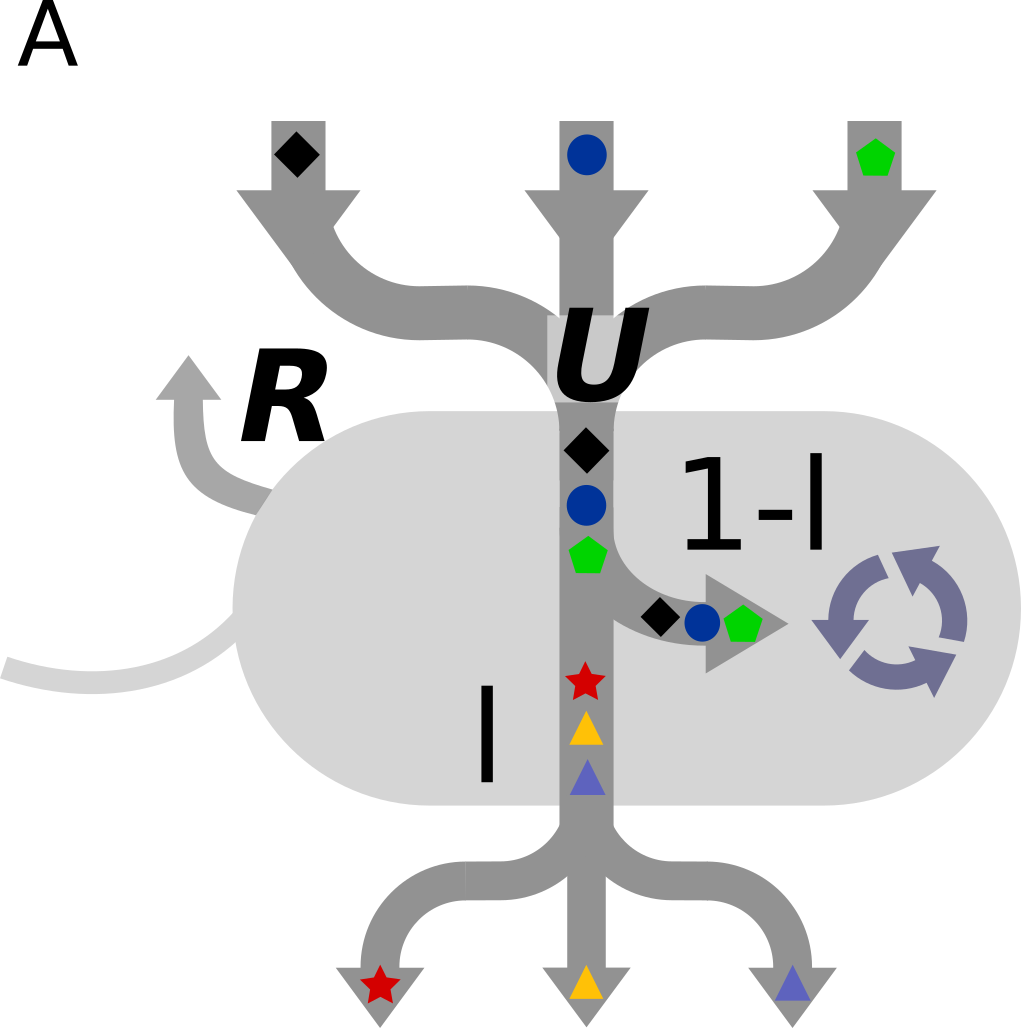
\includegraphics[scale=0.53]{./Figures/Model.png}
    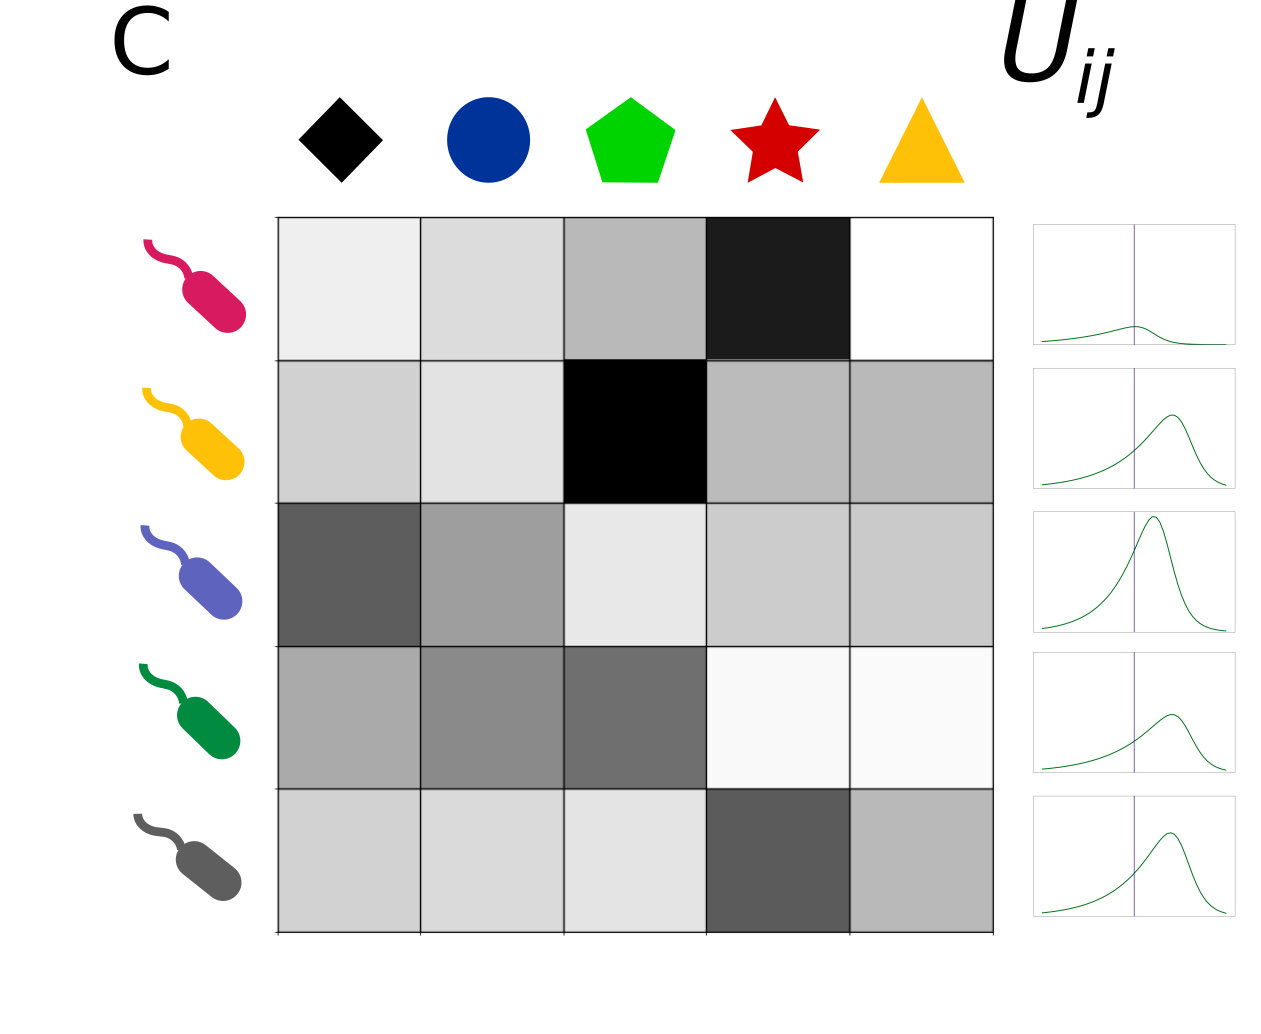
\includegraphics[scale=0.29]{./Figures/U.png}
    \end{tabular}
    \hfill
    \begin{tabular}{c@{}c@{}}
    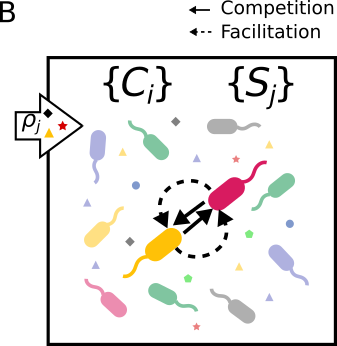
\includegraphics[scale=0.53]{./Figures/Community.png}
    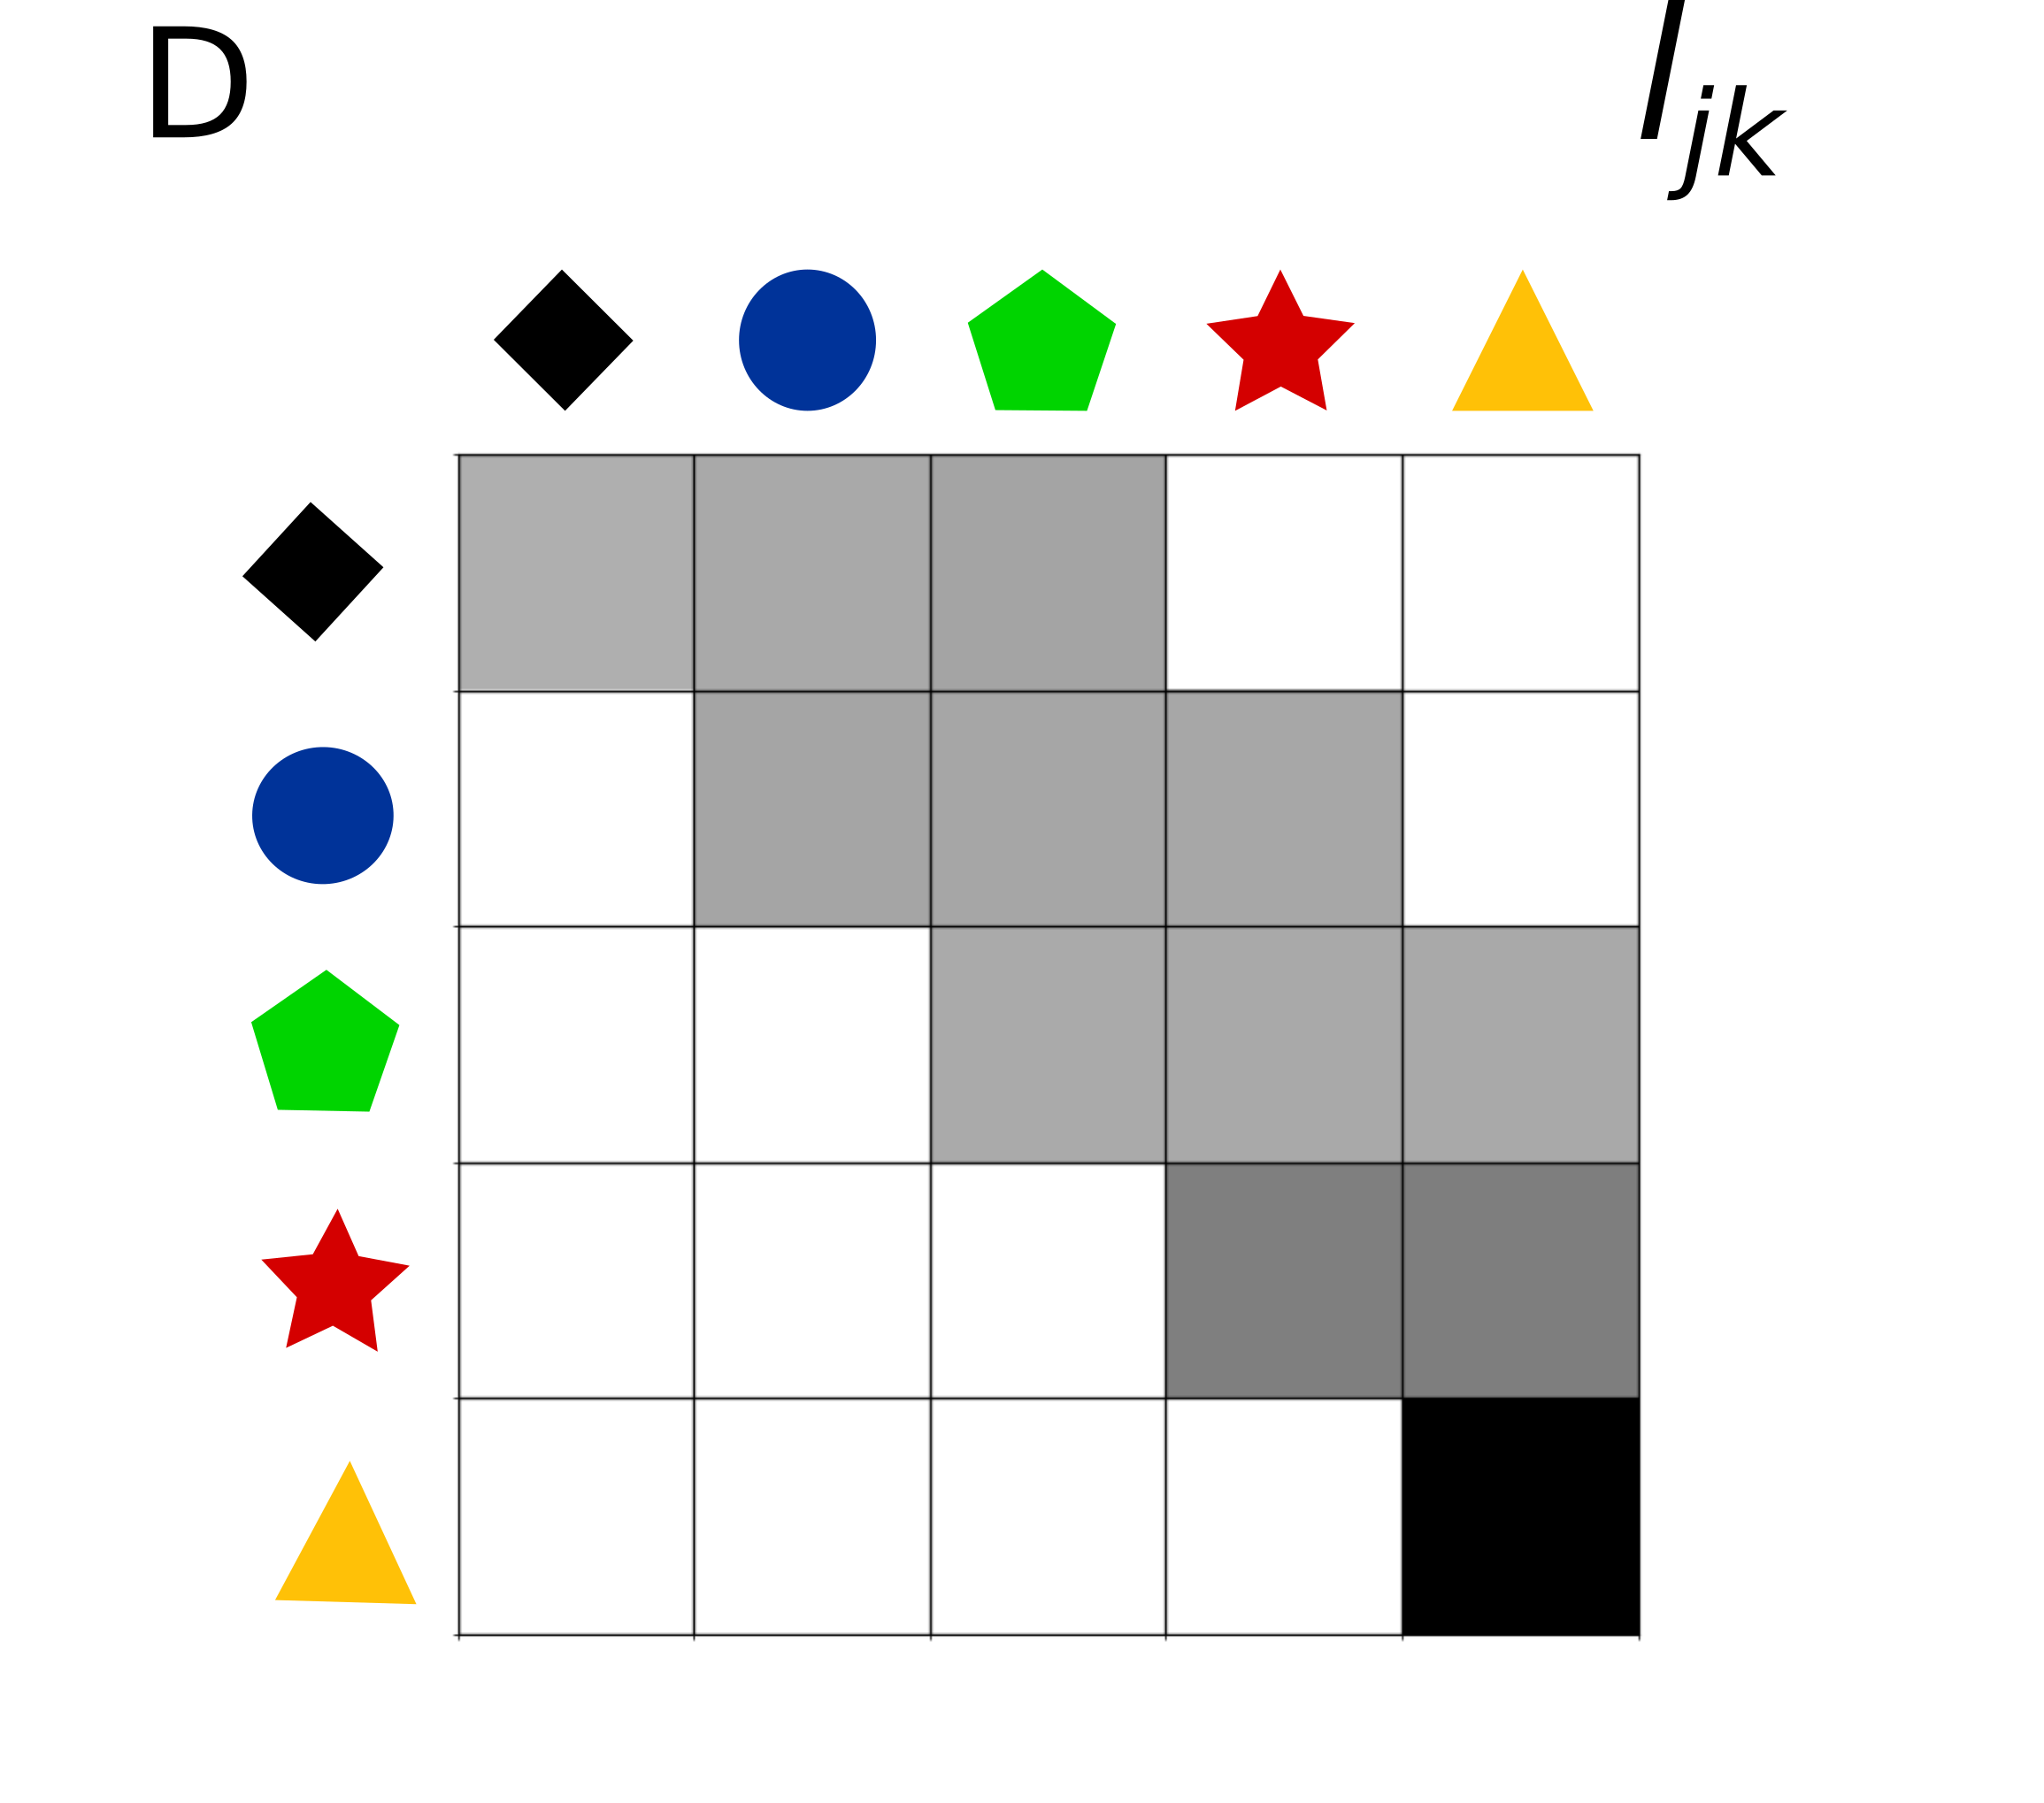
\includegraphics[scale=0.29]{./Figures/l.png}
    \end{tabular}
    \caption{\textbf{The microbial community model.} A: Schematic of the carbon fluxes in the microbial community model. The biomass concentration of consumers ($C_i$, $i$ = 1,2,...$N$) depends on the gain of carbon through resource uptake ($U$), minus the loss of carbon through leakage and the transformation of the intake carbon source ($l$) and maintenance respiration ($R$). B: Each microbial community is supplied with a constant and homogeneous inflow rate of all $M$ types of resources ($\rho_j$, $j$ = 1,2,...$M$), assuming the community is well-mixed so are all resources as soon as they enter the system. The resource concentration ($S_j$) of the system is modelled by abiotic external resource supply plus the biochemically transformed by-products through interspecies facilitation, minus the uptake of resources by consumers. C: Heat map of randomly sampled consumer preferential uptake rates matrix ($U_{ij}$) at 25\textdegree C (marked by the vertical lines in the TPCs displayed on the side), with $N = 5$ and $M = 5$. All resources uptake rates for each species are uniform random subsets of the species level uptake rate. D: Heat map of leakage-transformation matrix ($l_{jk}$) with $M = 5$. $l_{jk}$ governs the proportion of each consumed carbon resource released back into environment by either resource use inefficiency or the secretion of metabolic byproducts. In this leakage-transformation matrix (Figure \ref{fig:schematic}: D), when $j = k$, $l_{jj}$ represents the leakage fraction of resource $j$, which can be interpreted as resulting from the inefficiency of use of that resource. When $j < k$, $l_{jk}$ refers to the upper diagonal of this matrix, which fraction denotes the biochemical transformation of resource $j$ into other types of resource. Values are 0 for $l_{jk}$ when $j > k$ (in the lower diagonal), because we assume that reactions are irreversible, following the second law of thermodynamics. }
    \label{fig:schematic}
\end{figure}

\subsection{Temperature dependencies of parameters}\label{section:TPC}

The uptake and respiration rates follow the modified Sharpe-Schoolfield equation \citep{kontopoulos2020phytoplankton}:

\begin{align}\label{eq:U+R}
    U_i(T) = \frac{U_0\times {e^{\frac{-Ea_U}{k}\cdot\left(\frac{1}{T} - \frac{1}{T_{ref}}\right)}}}{1 + \frac{Ea_U}{E_{D_U}-Ea_U}e^{\frac{E_{D_U}}{k}\cdot(\frac{1}{T_{pk_U}}-\frac{1}{T})}}, \\
    R_i(T) = \frac{R_0 \times {e^{\frac{-Ea_R}{k}\cdot\left(\frac{1}{T} - \frac{1}{T_{ref}}\right)}}}{1 + \frac{Ea_R}{E_{D_R}-Ea_R}e^{\frac{E_{D_R}}{k}\cdot(\frac{1}{T_{pk_R}}-\frac{1}{T})}}.
\end{align}
Here, $T_{pk}$ is the optimum temperature for bacteria’s functional traits at which the metabolic rate peaks, $E_a$ is the activation energy, $E_D$ governs the decline rate of the traits when temperature exceeds $T_{pk}$. $T_{ref}$ is a reference temperature that allows the normalization constants $U_0$ and $R_0$ to be with the lowest variances among species, since the microbial metabolisms are governed by enzyme activities which performance are reduced at low temperature. As shown in the observation on species growth rates in Figure \ref{fig:G}A in Supplementary Information, the variance of species growth rates are lowest at $T_{ref}$ which is 0 \textdegree C. These normalization constants also include the scaling of the rate with cell size \citep{brown2004toward}. $T$ is the temperature for community assembly, which lies within the OTR. All parameters for the TPCs of the traits are listed in Table \ref{tab:T}. 

The Sharpe-Schoolfield equation is chosen here to approximate more realistic metabolic rates at all temperatures, however the results has proven to not be qualitatively dependent on the specific choice of TPC model as long as rates increase exponentially with temperatures within the OTR. 

\begin{table}
    \caption{Parameters for the temperature dependencies of uptake and respiration. $T_{pk_U}$ was sampled from a normal distribution with mean value at 308.15 $K$, and $T_{pk_R} = T_{pk_U} + 3$ to make sure species respiration always peak higher than uptake as is known to be the case in general \citep{smith2020systematic}. $E_a$ values were sampled from beta distributions with median values of 0.82 $eV$ and 0.67 $eV$ for uptake and respiration. $E_D$ values were set to 3.5 $eV$ for all reactions. A histogram of randomly sampled $E_a$ and $T_{pk}$ values are shown in Figure \ref{fig:SI_UR} in Supplementary Information. }
    \centering
    \begin{tabular}{ |m{3.3cm}<{\centering}|m{7cm}<{\centering}|m{1.5cm}<{\centering}|m{2.7cm}<{\centering}| } 
    \hline
     Parameter symbol & Parameter name & Units & Initial value \\
     \hline
    $U_0$ & Normalisation constant for uptake & - & 4.47 \\
    $R_0$ & Normalisation constant for respiration & - & 1.70 \\
    $Ea_U$ & Activation energy for uptake & eV & 0.82 \\
    $Ea_R$ & Activation energy for respiration & eV & 0.67 \\
    $k$ & Boltsmann constant & eV/K & $8.62$ $\times 10^{-5}$ \\
    $T$ & Model temperature & K & 273.15 \\
    $T_{ref}$ & Reference temperature & K & 273.15 \\
    $E_D$ & Deactivation energy & eV & 3.5 \\
    $T_{pk_U}$ & Peak temperature for uptake rate & K & 308.15 \\
    $T_{pk_R}$ & Peak temperature for uptake rate & K & 311.15 \\
    \hline
    \end{tabular}    
    \label{tab:T}
\end{table}

\subsection{Quantifying Carbon Use Efficiency }\label{section:CUE}

CUE---the proportion of harvested carbon allocated to cell growth---reflects the resource utilization ability of bacterial species. This is an intrinsic property for a species and is effectively its metabolic strategy for maximizing fitness.  I use the standard measure of CUE ($\frac{\text{Carbon Gain} - \text {Carbon Loss}}{\text{Carbon Gain}}$; \citep{manzoni2012environmental}) to calculate the intrinsic CUE for species $i$ given the above consumer-resource model (Equation \ref{eq:community}), which is:
\begin{equation}\label{eq:CUE_i}
CUE_i = \frac{\sum\limits _{j=1}^{M}U_{ij}S_j(1-\sum\limits_{k=1}^{M}l_{jk}) - R_i}{\sum\limits _{j=1}^{M}U_{ij}S_j}
\end{equation}
That is, CUE is the ratio (proportion) of carbon allocated to growth accounting for loss through respiration and leakage (production of metabolic byproducts though biochemical transformation of carbon resources) to that gained from uptake (the term in the denominator). 

Because the TPCs of underlying traits (Uptake and Respiration rate) within the OTR typically follow the Boltzmann-Arrhenius equation (numerator of Equation \ref{eq:U+R}), the TPC of species-level CUE within the OTR is well-approximated by the Boltzmann-Arrhenius equation \citep{smith2020systematic}:
\begin{equation*}
    CUE_i = CUE_0e^{-\frac{E_{a_{CUE}}}{k}(\frac{1}{T} - \frac{1}{T_{ref}})},
\end{equation*}
where the normalization constant $CUE_0$ is
\begin{equation}\label{eq:CUE0}
    CUE_0 = \frac{U_0(1 - l) - R_0}{U_0},
\end{equation}
And the apparent activation energy $E_{a_{CUE}}$ is 
\begin{equation}\label{eq:EaCUE}
    E_{a_{CUE}} = \frac{R_0(E_{a_U} - E_{a_R})}{U_0(1-l) - R_0}.
\end{equation}

Since $U_0$, $R_0$ and $l$ ($l$ here denote the total carbon use inefficiency for each resource during uptake) are constants across species in the simulation, the thermal sensitivity of CUE is solely dependent on the differences between $E_U$ and $E_R$. Therefore, in this case, if the species’ respiration has higher thermal sensitivity than its uptake ($E_{a_R} > E_{a_U}$), then high temperature is unfavourable for the species' growth. This species would have a CUE thermal response (negative $E_{a_{CUE}}$), which means that the species' resource utilization ability decreases with rising temperature. 

\subsection{Quantifying pair-wise species interactions}

Inter-species interactions are also deterministic factors for the number of coexisting species in a microbial community. In terms of species' carbon resource utilization, pairwise interactions of all species in the community are either competitive or facilitative. 

Since all species in a community exploit the same pool of carbon resources, the pair-wise resources competition can be quantified by the overlap in their resource use. Here I use the weighted Jaccard similarity coefficient  ($J_c$) to measure this overlap, which for a species pair $\alpha$ and $\beta$ is: 
\begin{equation*}\label{eq:c}
    J_c = \frac{\sum\limits_{j=1}^M \min (U_{\alpha j},U_{\beta j})}{\sum\limits_{j=1}^M \max (U_{\alpha j},U_{\beta j})}.
\end{equation*}
The resulting $N \times N$ pair-wise competition matrix (Figure \ref{fig:J}A) is symmetric with 1's on the diagonal, as the resource overlap is bidirectional between species. I then take average values by columns to get the average resource overlaps of one species and all the others. Since the pair-wise competition matrix is symmetric, taking the average by either a row or column of the matrix would provide the same result.

Cross-feeding describes the metabolic products of one species which can be consumed as resources by another species. To quantify facilitation though cross-feeding between species in a community, for a species pair $\alpha$ and $\beta$, I calculate the overlap of the leakage and transformation of resources by species $\alpha$ and the uptake rates vector of species $\beta$ as:
\begin{equation*}\label{eq:f}
    J_f = \frac{\sum\limits_{j=1}^M \min\left(\sum\limits_{k=1}^M U_{\alpha k}l_{kj},U_{\beta j}\right)}{\sum\limits_{j=1}^M \max\left(\sum\limits_{k=1}^M U_{\alpha k}l_{kj},U_{\beta j}\right)}.
\end{equation*}
In contrast to the competition matrix, the $N \times N$ facilitation matrix (Figure \ref{fig:J}: B) is asymmetric because cross-feeding is directional. The rate of metabolite production by one consumer is dependent both on its uptake and ability for resource transformation. I take the mean values of all columns (row-wise), which gives the quantification of the ability of each species for promoting facilitative interactions. 

\begin{figure}
    \centering
    \begin{tabular}{c@{}c@{}}
    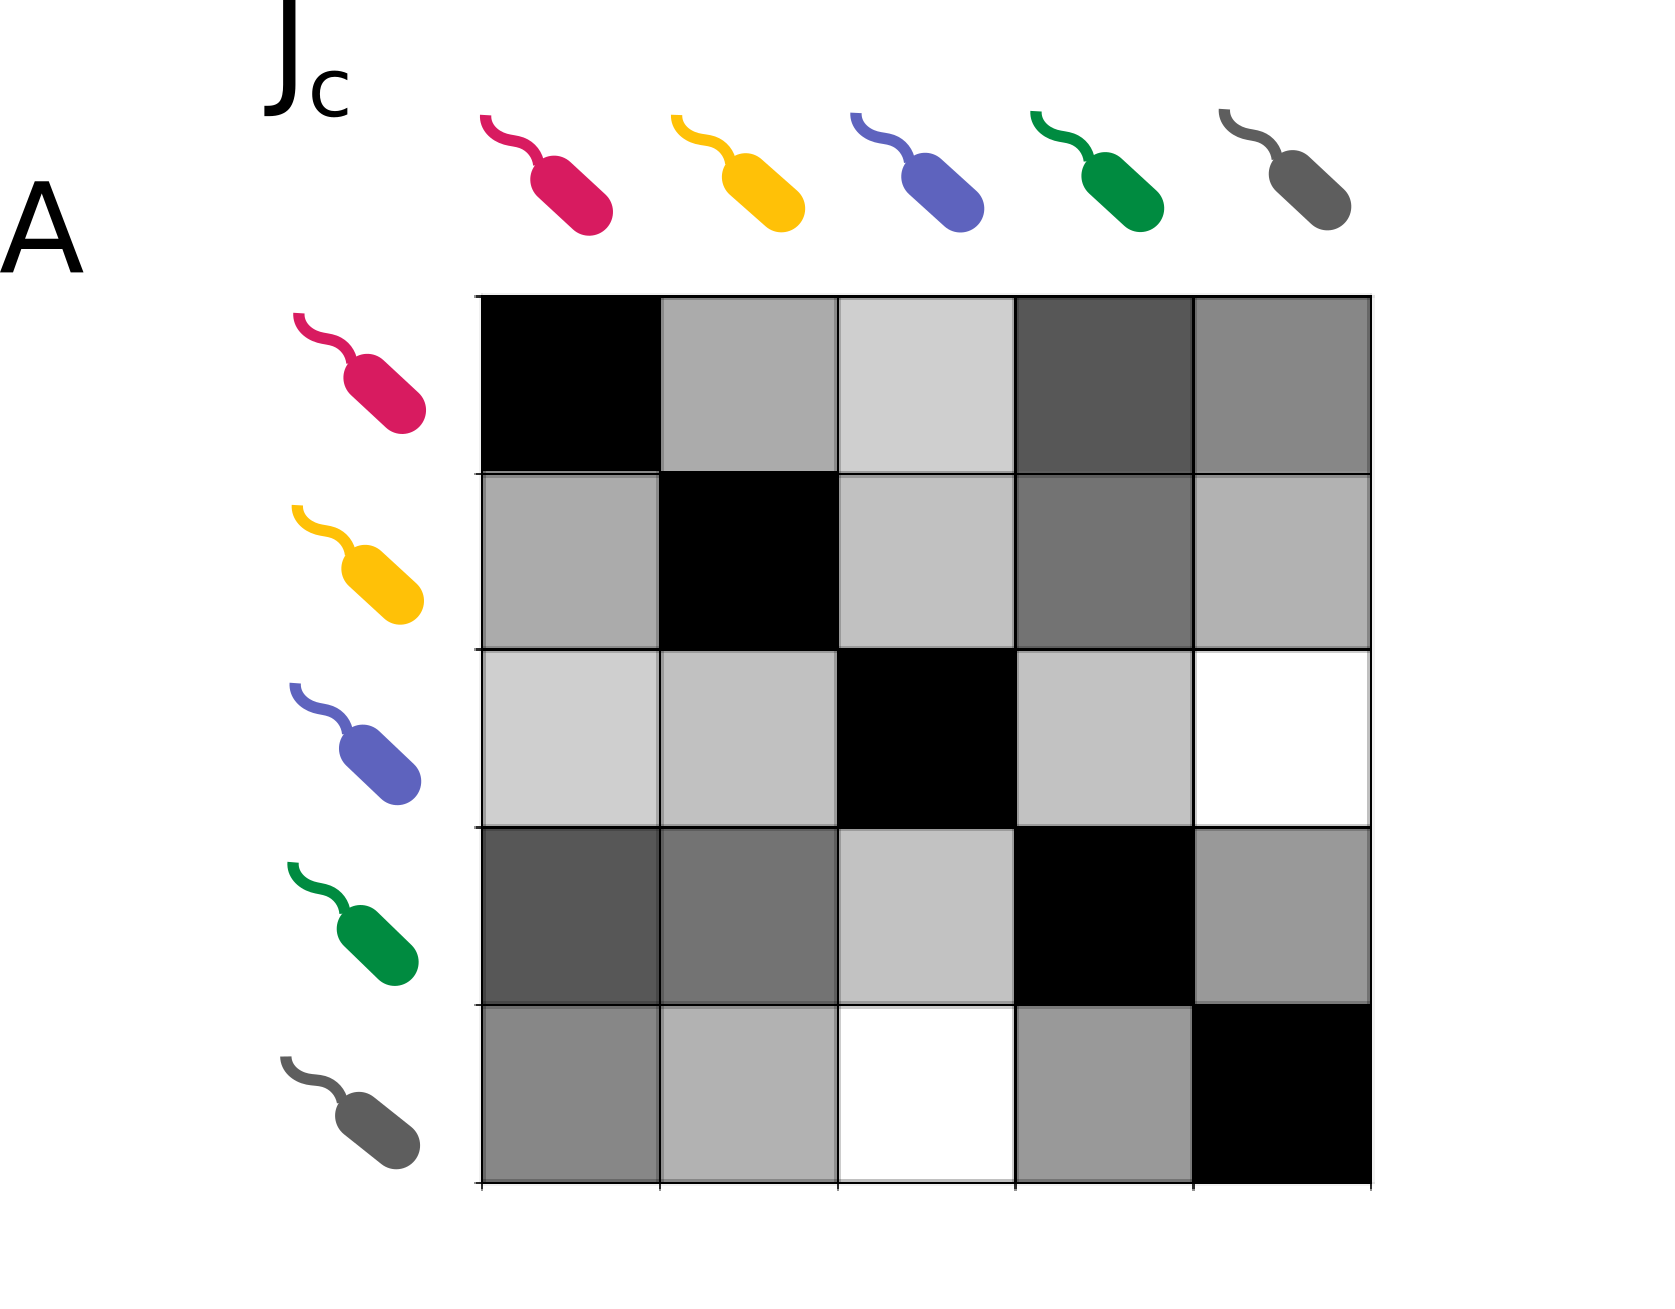
\includegraphics[scale=0.45]{./Figures/Jc.png}
    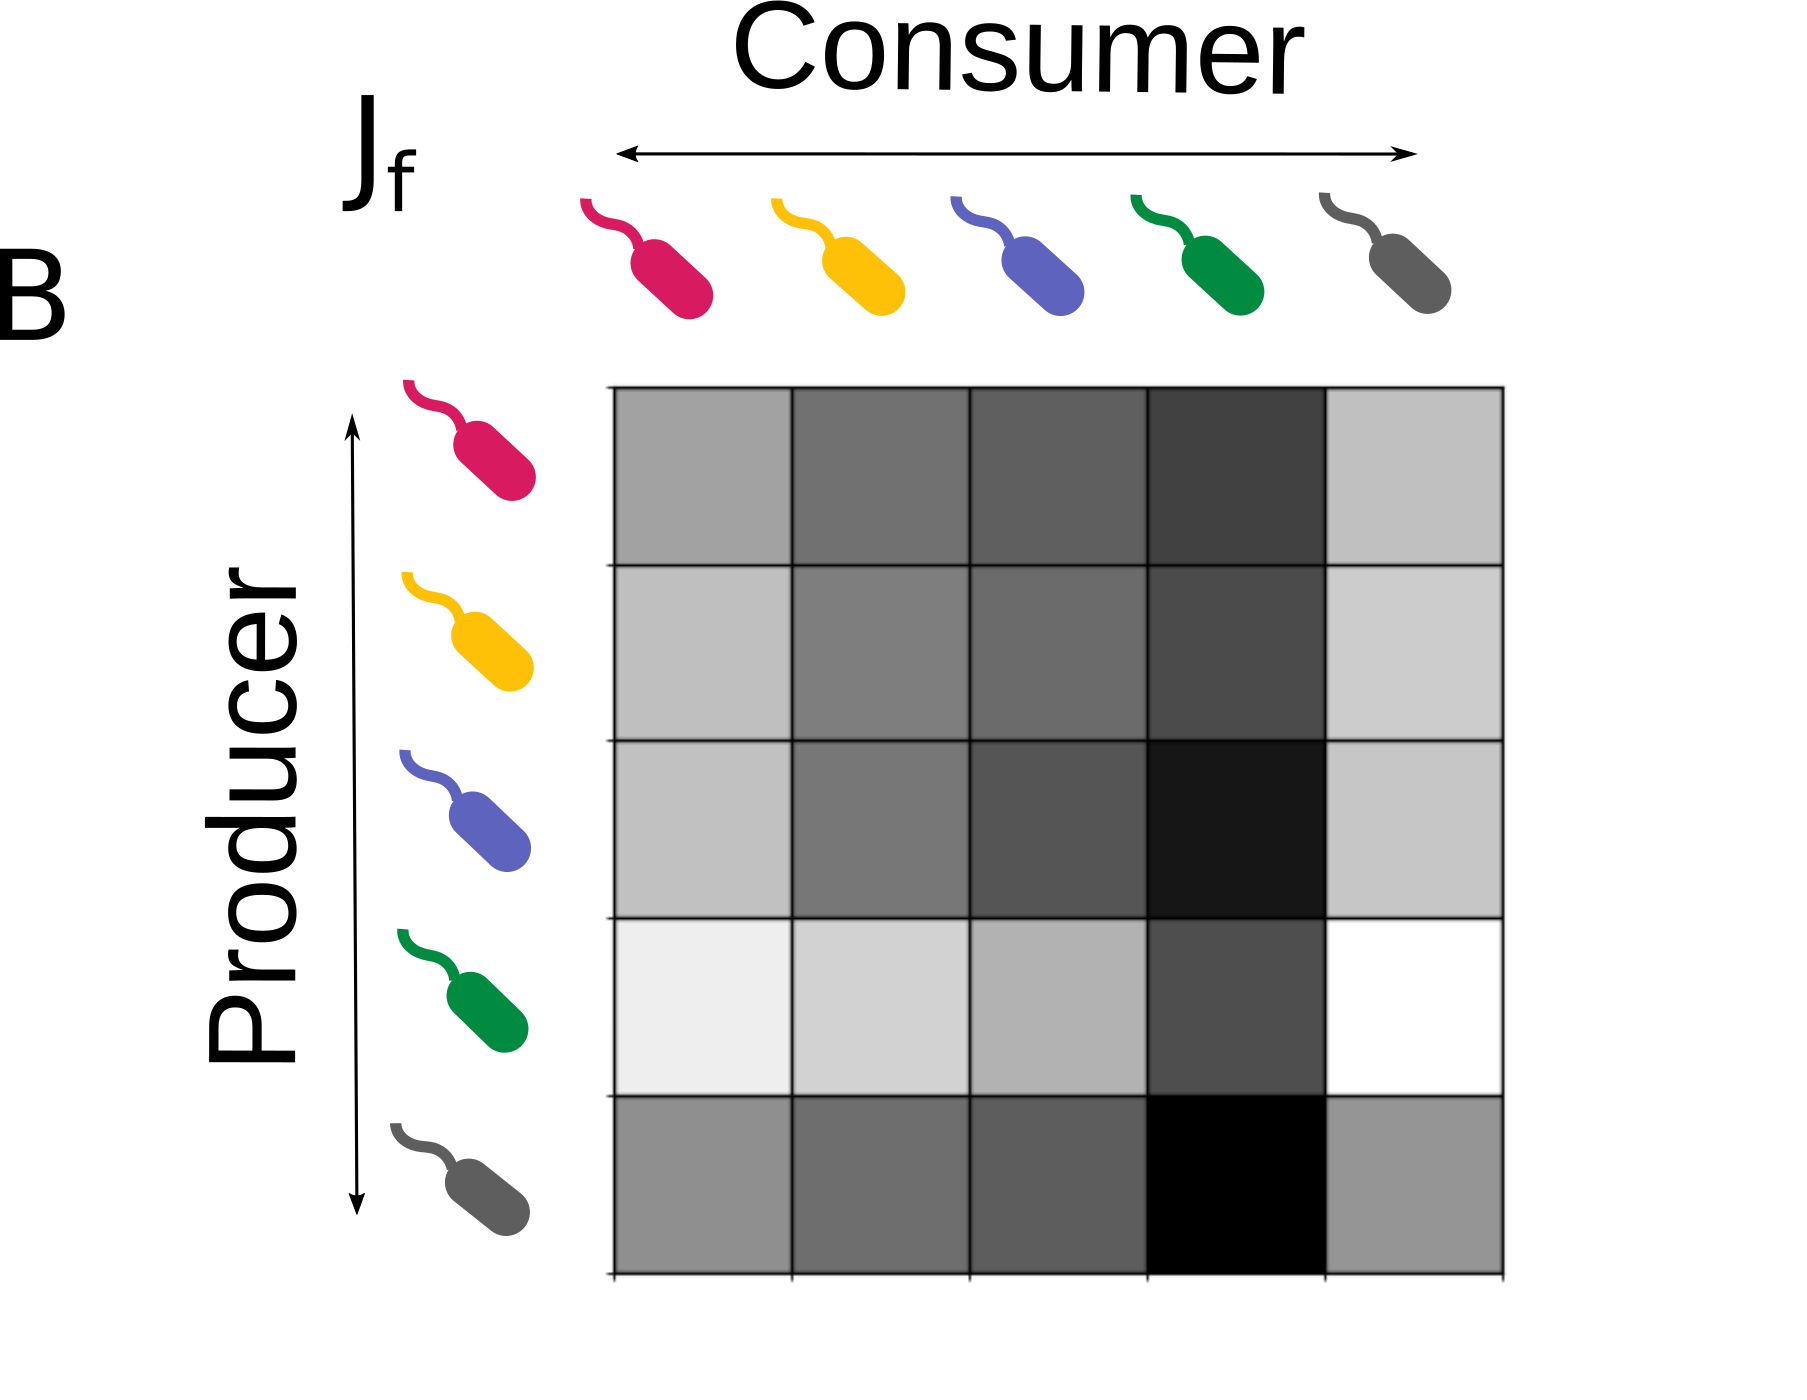
\includegraphics[scale=0.45]{./Figures/Jf.png}
    \end{tabular}
    \caption{\textbf{Illustration of the pairwise species interaction matrices for a $N=5$ community}. A: Competition matrix ($J_c$). B: Facilitation matrix ($J_f$). Species acting as metabolic byproduct producers are along the rows, and those acting as consumers of these metabolic by products along columns. }
    \label{fig:J}
\end{figure}

\subsection{Community assembly simulations}

To investigate the effect of temperature on species richness, I simulated community assembly based on equation \ref{eq:community} with a random pool of 100 species competing for 50 carbon resources, and parameter values as described in the previous sections. For each assembly simulation, I numerically integrated the ODE system for 4000 time-steps, by which time every community reached dynamic equilibrium (where $dC_i/dt = 0$ and $dS_j/dt = 0$), i.e., the surviving species coexisted. 

For each species, the uptake rates ($U_{ij}$) of all resources are uniform random subsets of the species level uptake rate ($U_i$). I used Dirichlet distribution for assigning these resources uptake rates with $\alpha = 1$, therefore all subset uptake rates of $M$ resources sum up to the species level uptake rate (Figure \ref{fig:schematic} C). $U_{ij}(T)$ also contains the functional response of resource uptake with resource concentration. Here, I focus on the linear functional response of species growth with resource concentration, but my results still hold with resource uptake as Monod (Type II) functional response (Figure \ref{fig:TypeII} in Supplementary Information). 

I parameterized the species' TPCs using empirical data from \cite{smith2019community, smith2020systematic}, using $E_a$ values for species growth rates as proxy for $E_a$ values for resource uptake rates. Empirical data on the thermal sensitivities of resource uptake rates are lacking, therefore I assumed similar thermal sensitivities for uptake as those for growth rate. This is a reasonable assumption because the metabolic mechanisms of the resource uptake by species mainly governs the maximum growth rates of microbial species. Figure \ref{fig:G}A in Supplementary Information shows the TPCs of lab cultured bacterial growth rates collected and standardized in \cite{smith2019community}, which contains $N = 377$ individual growth rate temperature performance curves after filtering. A set of resource uptake and respiration rates of $M = 50$ and $N = 100$ is shown in Figure \ref{fig:G}B \& C in Supplementary Information.

The $U_0$ and $R_0$ values at 0 \textdegree C are calculated combining my CUE calculation (refer to equation \ref{eq:CUE0} in section \ref{section:CUE}) with another conventional CUE calculation method, and the $CUE_0 = 0.22$ ($CUE_0$ denotes the median CUE value at reference temperature) as in \cite{smith2020systematic}, where resource uptake is assumed to be mainly allocated to growth and respiration ($U \approx R + \mu$, where $\mu$ denotes the growth rate of the species):

\begin{equation*}
    CUE_0 = \frac{\mu_0}{\mu_0 + R_0} = \frac{U_0(1-l) - R_0}{U_0} = 0.22
\end{equation*}
As the mean growth rates at $T = 0$ \textdegree C ($\mu_0$) is 0.48 according to \cite{smith2019community}, I set $B_U$ and $B_R$ to be 4.47 (unit: 1/time) and 1.70 (unit: mass/volume$\cdot$time) in the TPCs of uptake and respiration rates. 

The richness value of the community was recorded at the end of each simulation as the number of species with biomass abundance $C_i > 0$. I also recorded the uptake and respiration rate, CUE, $E_{a_{CUE}}$ and $S^*$ of each species, and pair-wise species interaction indexes ($J_c$ \& $J_f$) in the community for each simulation. I calculate carbon uptake using the starting values of resources concentration ($S_j = S_{j0} = 1$), neglecting the fluctuation of resources concentration derived from interspecies competition and facilitation during assembly. This assembly simulation procedure was replicated 30 times at each temperatures from 0-30 \textdegree C. This temperature range covered the OTR of most species (Figure \ref{fig:G} in Supplementary Information), i.e., did not allow high temperature effects to come into play for most species. 

Further, to test the effects of facilitation (leakage) on species richness patterns across temperatures, I fixed the leakage fraction of each resource to 0, 0.1, 0.3, 0.5 and 0.7. Then the simulation was run for 50 assemblies for each one of these leakage fractions. 

All simulations of community assemblies are run using Python. \texttt{Numpy} package \citep{harris2020array} is used for array and matrices manipulation and random values generation. The \texttt{odient} function from \texttt{scipy.integrate} \citep{virtanen2020scipy} is used for numerical integration. Figures are plotted using \texttt{Matplotlib} \citep{Hunter:2007}. An example of resource and consumer dynamics of 100 species at the reference temperature is shown in Figure \ref{fig:example} in Supplementary Information. 

\section{Results}

Figure \ref{fig:rich}A shows that species richness declines with increasing temperature within OTR. I explain this pattern from two perspectives: the role of species' metabolic strategies in species sorting and the relative importance of interspecies interactions at different temperatures.

\subsection{The role of species' metabolic strategies in species sorting}

Figure \ref{fig:rich}B shows the pattern of change in microbial community species richness at equilibrium following assembly for an example community. The species richness of the system declines because the environment cannot sustain the coexistence of more consumers than resources at steady state based on the competitive exclusion theory \citep{hardin1960competitive, levin1970community}. I numerically explain the filtering of metabolic strategies in species sorting by considering the competitive exclusion of species using the $R^*$ rule, that is when two species are competing over one resource, the winner would be the one with lower resource requirement for growth when the system reaches equilibrium regardless of species initial biomass \citep{tilman1982resource}, because the resource concentration at steady state would not suffice the growth of the other species with higher equilibrium resource requirement. Figure \ref{fig:2_example} in Supplementary Information shows the examples of this competition. At 0 \textdegree C, since both species have the same equilibrium resource requirement, the coexistence of both species can be achieved at equilibrium. At temperatures higher than $T_{ref}$, species have different resource requirements, so the species with relatively higher resource requirement are outcompeted therefore extinct before reaching equilibrium. 

\begin{figure}
    \centering
    \begin{tabular}{c@{}c@{}}
    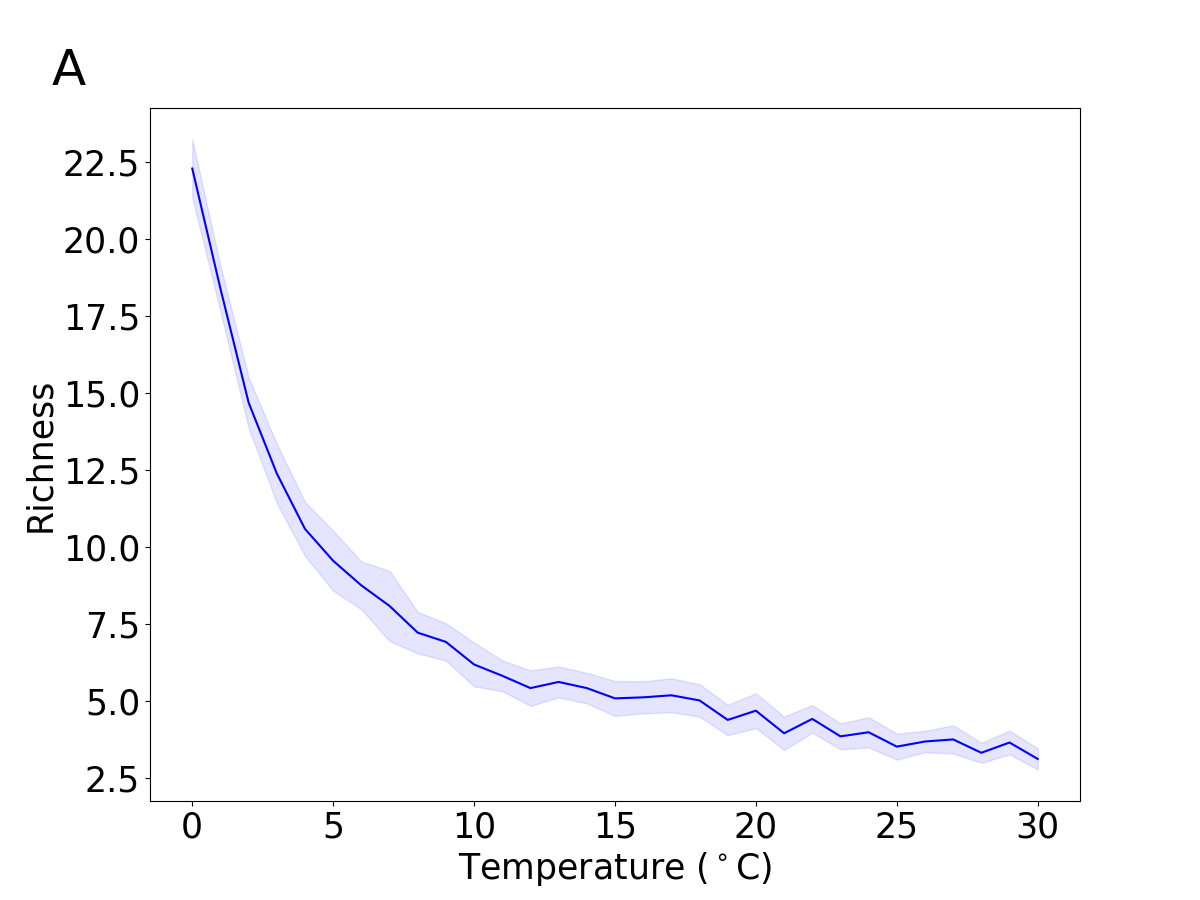
\includegraphics[scale=0.27]{./Figures/selectingEaCUE.png}
    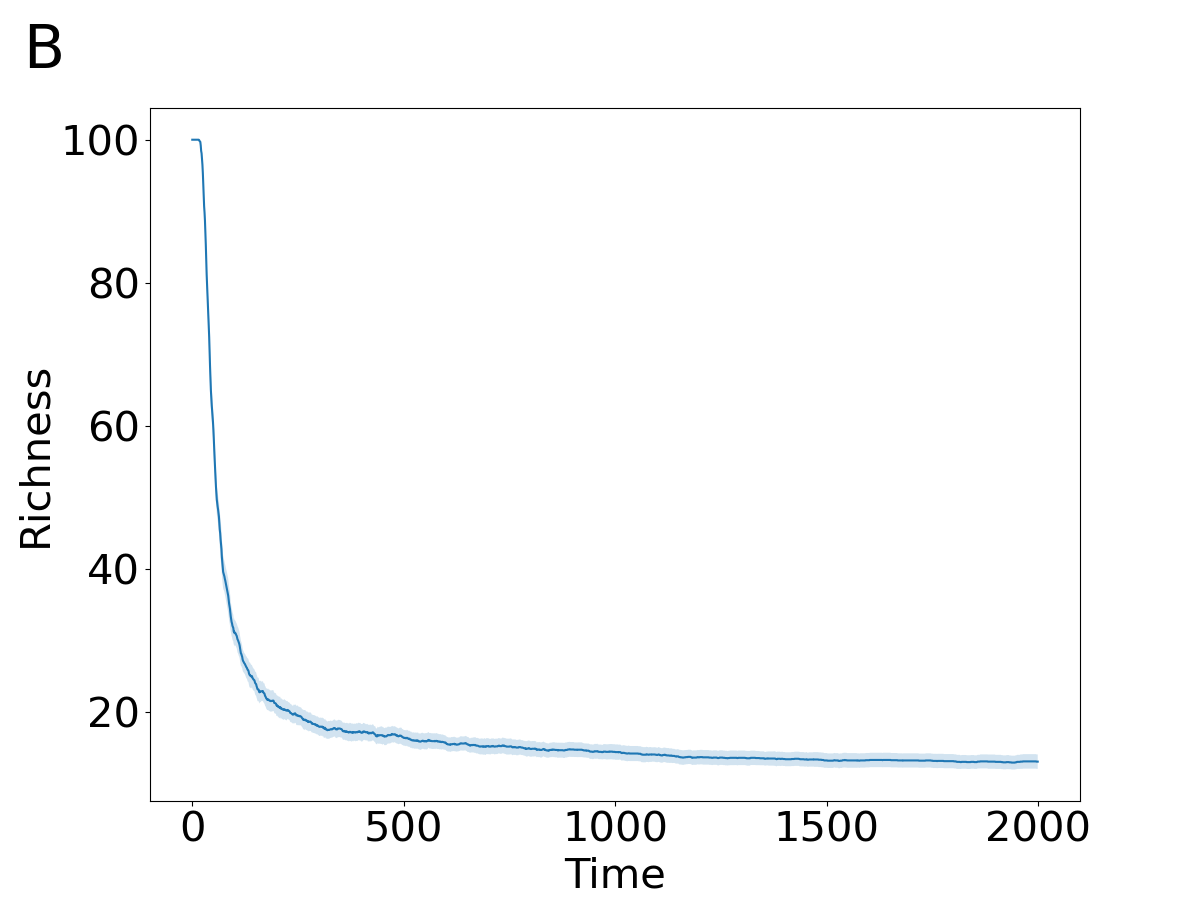
\includegraphics[scale=0.27]{./Figures/rich_decay.png}
    \end{tabular}
    \caption{\textbf{Patterns in community diversity and structure emerging from species sorting at different temperatures.} A: Species richness of communities assembled under different temperatures within the OTR, plotted with $0.95 \%$ confidence interval (CI) bands of all 30 communities richness values at each temperature. B: Change in microbial community diversity during assembly at a fixed temperature. This plot shows the average richness with $0.95 \%$ confidence interval (CI) bands of 30 replicated assembly simulations at reference temperature ($0 ^\circ$C). }
    \label{fig:rich}
\end{figure}

If consider these species growing independently, according to the $R^*$ rule, the equilibrium resource requirement for species growth of the $i^{th}$ species $S^*_i$ can be calculated as: 
\begin{equation}\label{eq:S*}
S^*_i = \frac{R_i}{U_i(1-l)}
\end{equation}

\begin{figure}
    \centering
    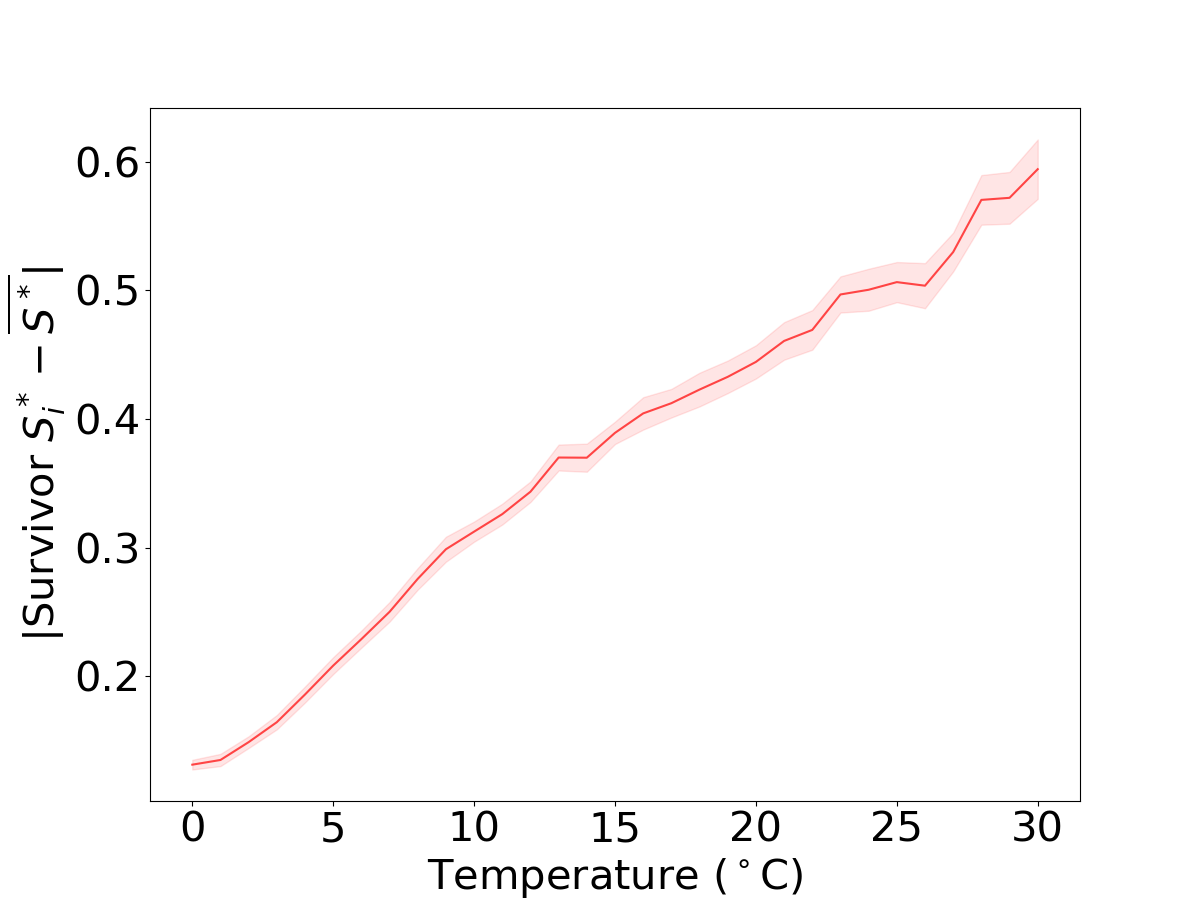
\includegraphics[scale=0.3]{./Figures/eq_st.png}
    \caption{\textbf{The magnitude of competitive exclusion at different temperatures.} This plot shows the increasing "strength" of excluding higher $S^*$ species with temperature, calculated by the $S^*$ differences between survivors and community average $S^*$ as $|S_i^* - \overline{S^*}|$. The band shows the 95\% CI of the relative survivor $S^*$ values at each temperature.}
    \label{fig:Sdiff}
\end{figure}

Since I consider species sorting as a result of competitive exclusion under different temperatures where species with higher $S^*$ are eliminated. I quantified the magnitude of this competitive exclusion at different temperatures by calculating the $S^*$ differences between survivors and community average $S^*$ as $|S_i^* - \overline{S^*}|$. As shown in Figure \ref{fig:Sdiff}, the magnitude of excluding high $S^*$ species increased with temperature. Here I numerically show how the filtering on species' metabolic strategies ($CUE$ and $E_{a_{CUE}}$) is relevant to this competitive exclusion of species. The numerical link between species $CUE$ and resource requirement for the $i^{th}$ species ($S^*_i$):
\begin{equation}\label{eq:S_CUE}
CUE_i = (1 - S^*_i) (1-l)
\end{equation}
Therefore, the advantage of lower resource requirement in resource competition is equivalent to having higher intrinsic CUE values. 

As shown in Figure \ref{fig:CUE}A, as temperature increases, both resource uptake rates and maintenance respiration rates increase exponentially following equation \ref{eq:U+R}. And since $E_{a_U} > E_{a_R}$, the increase of uptake rates with temperature exceeds that of respiration with temperature. Species with higher uptake rates and lower respiration rates are favored in species sorting at all temperatures as shown in Figure \ref{fig:CUE}A. The combination of these is the exponential increase of species intrinsic CUE (equation \ref{eq:CUE_i}), and the advantage for species with higher intrinsic CUE in succeeding resource competitions at all temperatures (Figure \ref{fig:CUE}B). 

\begin{figure}
    \centering
    \begin{tabular}{c@{}c@{}}
    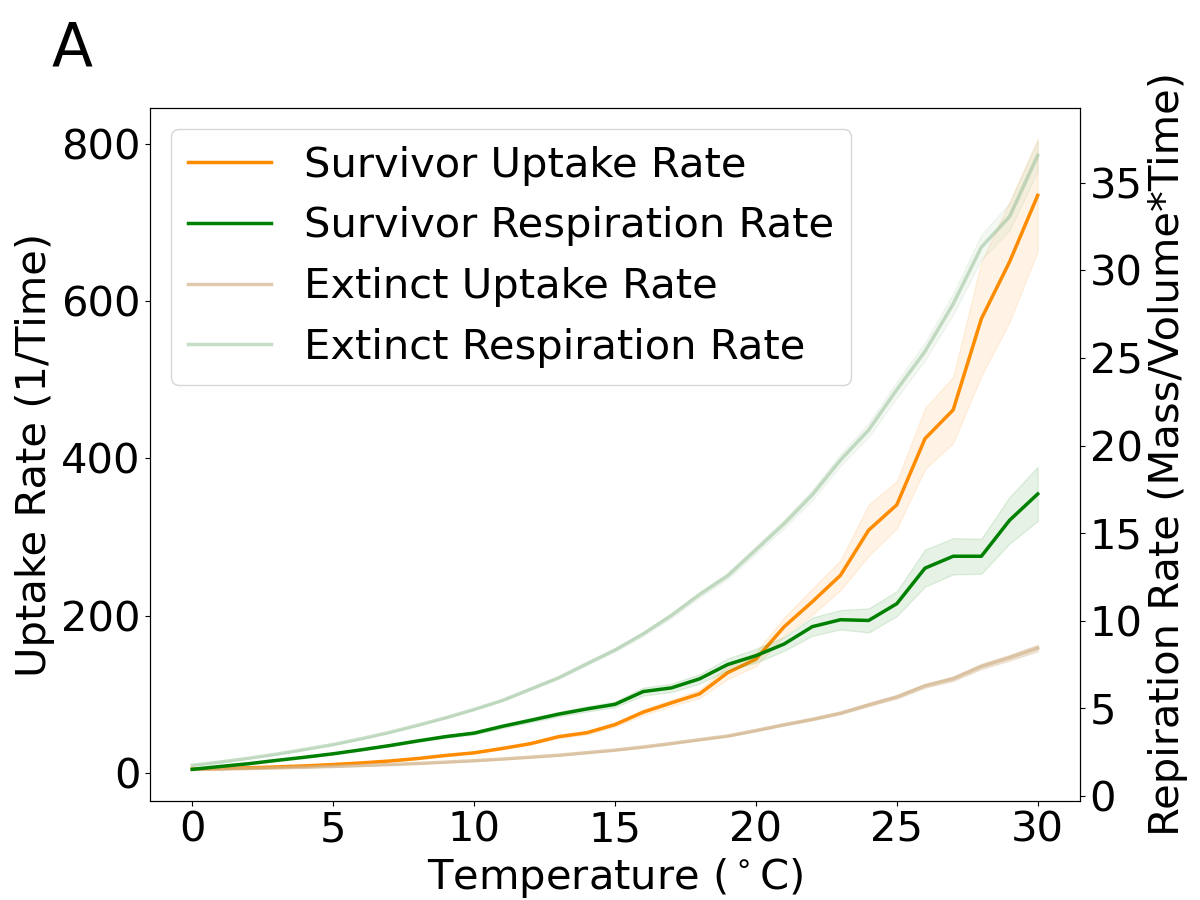
\includegraphics[scale=0.27]{./Figures/selectingEaCUE_1.png}
    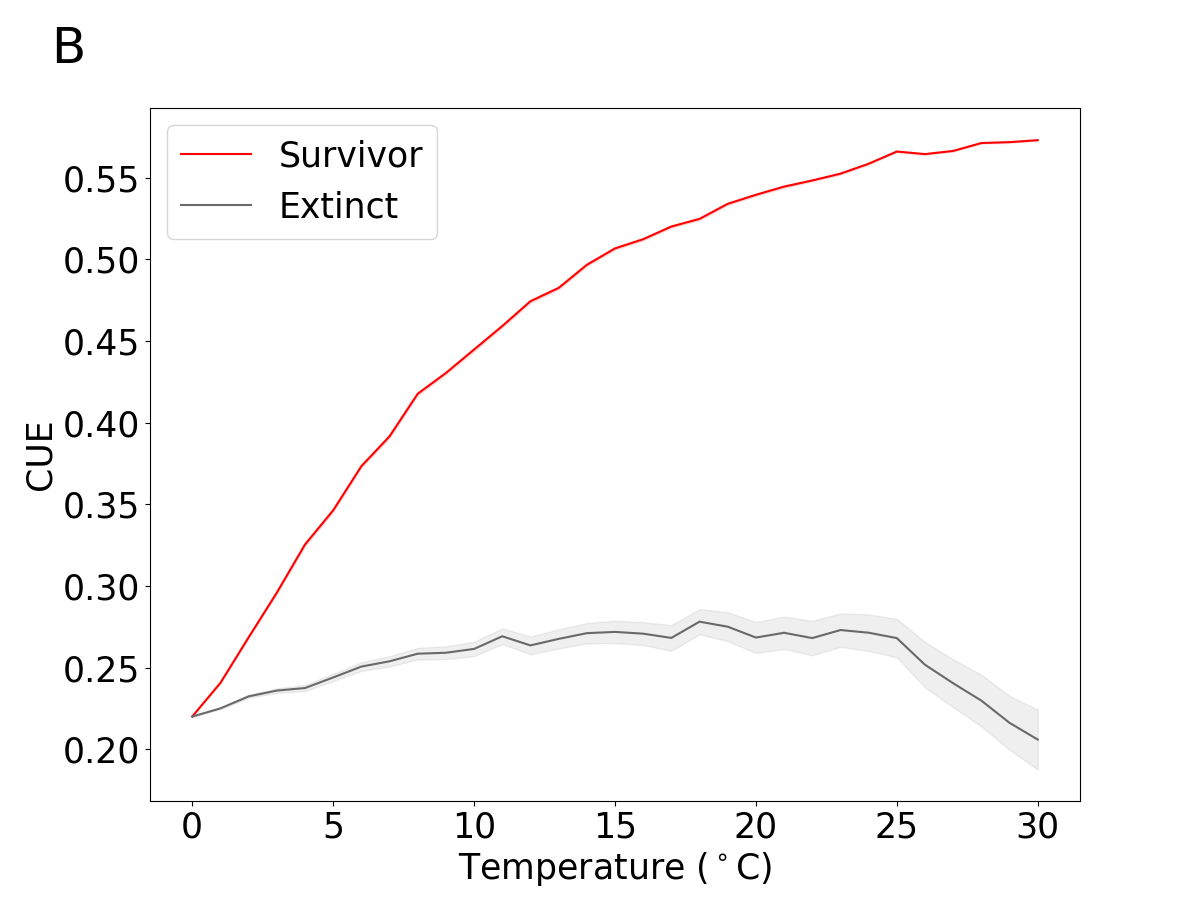
\includegraphics[scale=0.27]{./Figures/selectingEaCUE_2.png}
    \end{tabular}
    \caption{\textbf{Patterns in species CUE emerging from species sorting during community assemblies at different temperatures.} A: The exponential increase in uptake and respiration rates of survivors and extinct species in communities assembled at different temperatures. B: The emergent intrinsic CUEs of survivors and extinct species in communities assembled at different temperatures. The bands denote 95\% CIs of the survivors and extinct species uptake and respiration rates (B) and intrinsic CUEs (C) of 30 assemblies at each temperature. }
    \label{fig:CUE}
\end{figure}

The numerical link between species $S^*$ and $E_{a_{CUE}}$ for the $i^{th}$ species is as follow:
\begin{equation}\label{eq:S_Ea}
lnS^*_i = lnR_0 - ln(1-l)U_0 + \frac{U_0(1-l) - R_0}{R_0}E_{a_{CUE}}\Delta T
\end{equation}
Therefore, species with lower $S^*$ values also have higher $E_{a_{CUE}}$ (Figure \ref{fig:EaCUE}A). The derivation of these two equations is shown in Supplementary Information (Section \ref{sec:S+CUE}). The increasing magnitude of competitive exclusion also shows as the increasing elimination of species with relatively lower $E_{a_{CUE}}$ at higher temperatures (Figure \ref{fig:EaCUE}B). As shown in Figure \ref{fig:EaCUE}B, survivors' $E_{a_{CUE}}$ shows a linear negative correlation with species richness. This indicates that species sorting governed by competitive exclusion is the major driver for the species richness decline in communities assembled at increasing temperatures. 

\begin{figure}
    \centering
    \begin{tabular}{c@{}c@{}}
        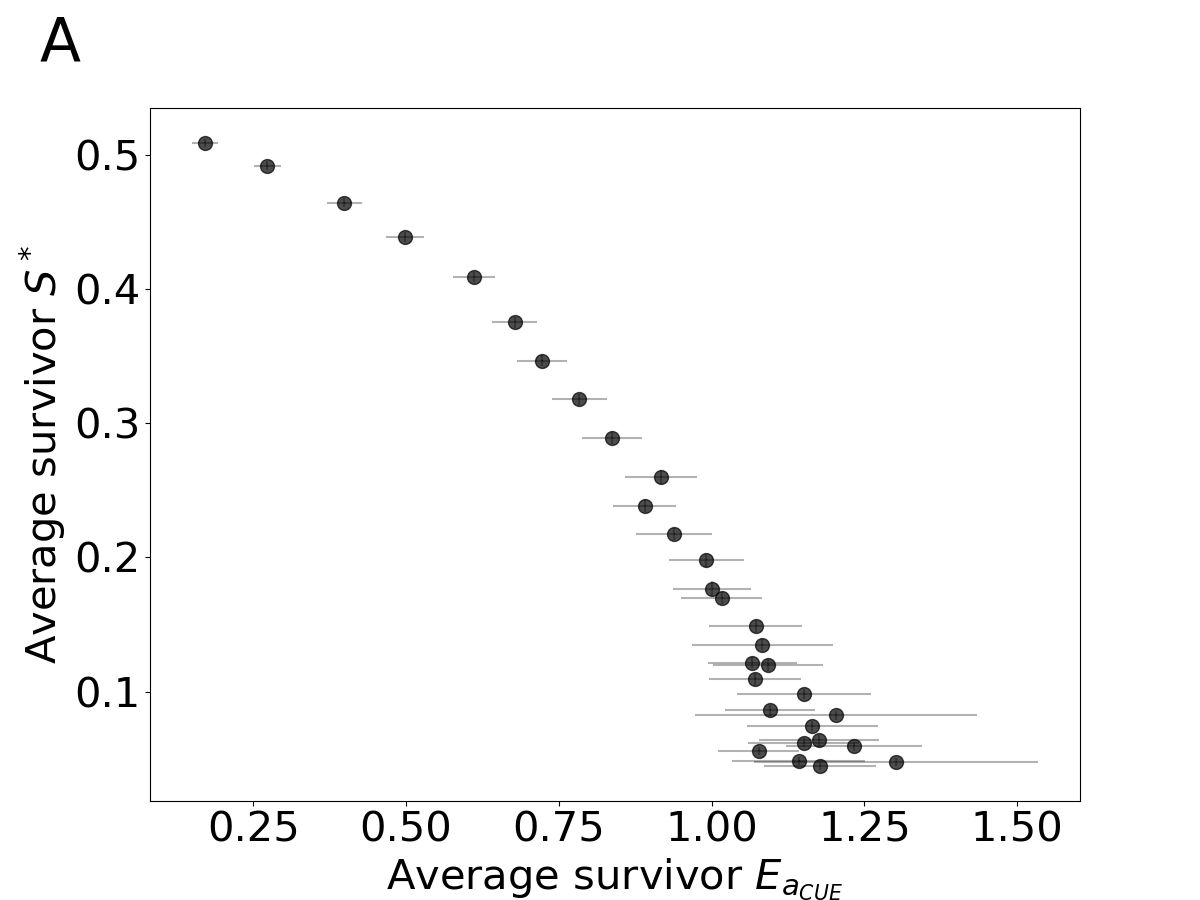
\includegraphics[scale=0.27]{./Figures/Eadiff_fitdiff.png}
        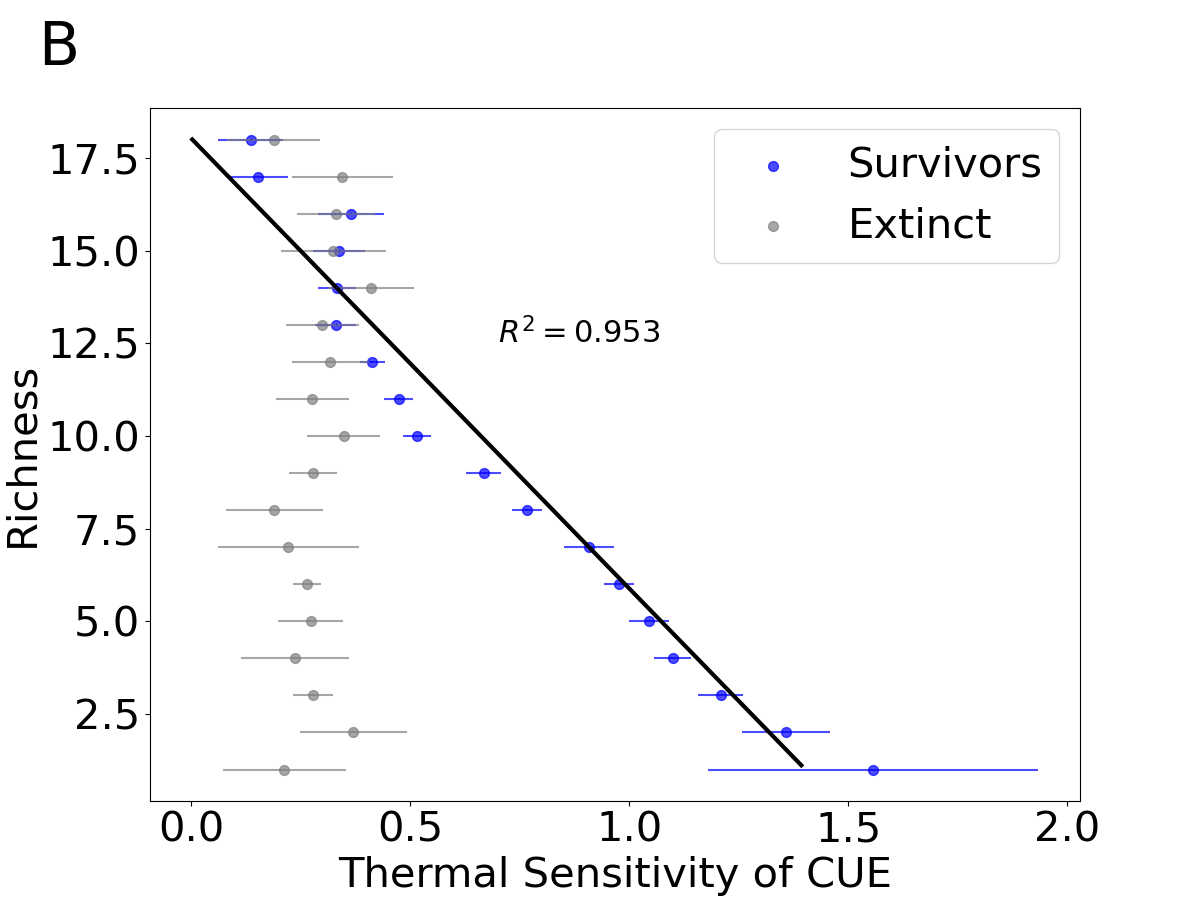
\includegraphics[scale=0.27]{./Figures/EaCUE_richness.png}
    \end{tabular}
    \caption{\textbf{Species sorting based on species $E_{a_{CUE}}$ plays the definitive role in species richness at different temperatures.} A: The negative correlation between average survivors' $S^*$ and $E_{a_{CUE}}$. Plotted using the all survivor $S^*$ and $E_{a_{CUE}}$ values of 30 parallel communities assembled at all temperatures, error bars are plotted at CI = 95\%. B: The relation between species richness and the thermal sensitivities of species CUE ($E_{a_{CUE}}$). Plotted using the richness values of all 30 parallel communities assembled at all temperatures. The black line shows the linear negative correlation of community richness and average survivors' $E_{a_{CUE}}$ in the community as the result of species sorting, with $R^2 = 0.946$.}
    \label{fig:EaCUE}
\end{figure}

\subsection{Interspecies interactions at different temperatures}

Figure \ref{fig:cf}A shows that both (community-level) resource overlap and cross-feeding decrease with increasing temperature. In general, species with less resource overlaps and higher facilitation ability are favored especially at high temperatures. However the positive effect of facilitation on richness is outweighted by the decreasing resource overlap (increasing niche partioning) of survivors beyond a temperature range of 10-15 \textdegree C. The variance in resource uptake (Figure \ref{fig:cf}B) for each species depicts this species differential resource uptake rates among $M$ resources. Specifically, if a species have higher variance in resource uptake, it means that this species have distinctively higher uptake rates of few specific resources and distinctively lower of the rest. Whereas if a species have low variance in resource uptake, meaning this species generally uptake all $M$ at a relatively similar rate without preferences. The high existence of species with low variance in resource uptake would result in higher resources overlap among species. As shown in Figure \ref{fig:cf}B, species with higher variance in resource uptake are favored also starting around 10-15 \textdegree C.

\begin{figure}
    \centering
    \begin{tabular}{c@{}c@{}}
    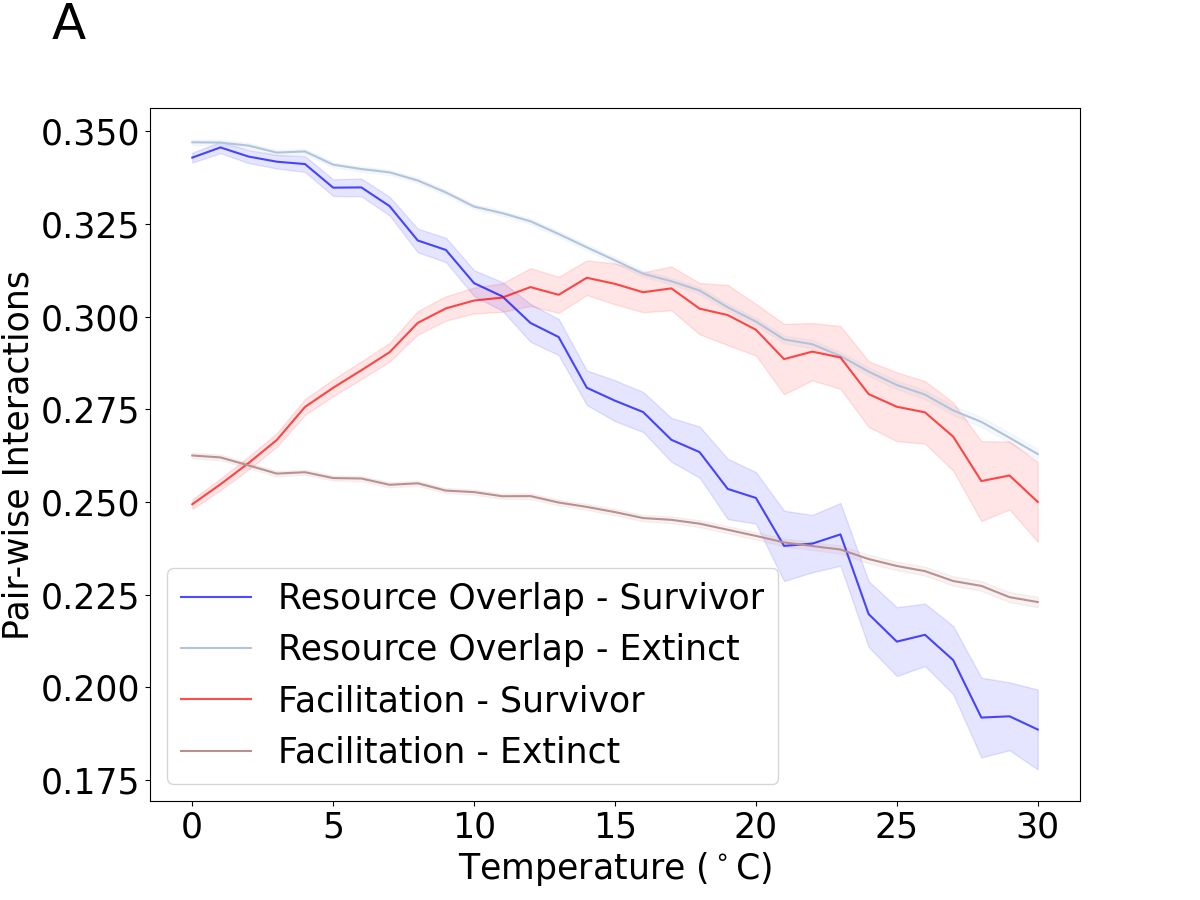
\includegraphics[scale=0.27]{./Figures/Resource_overlap.png}
    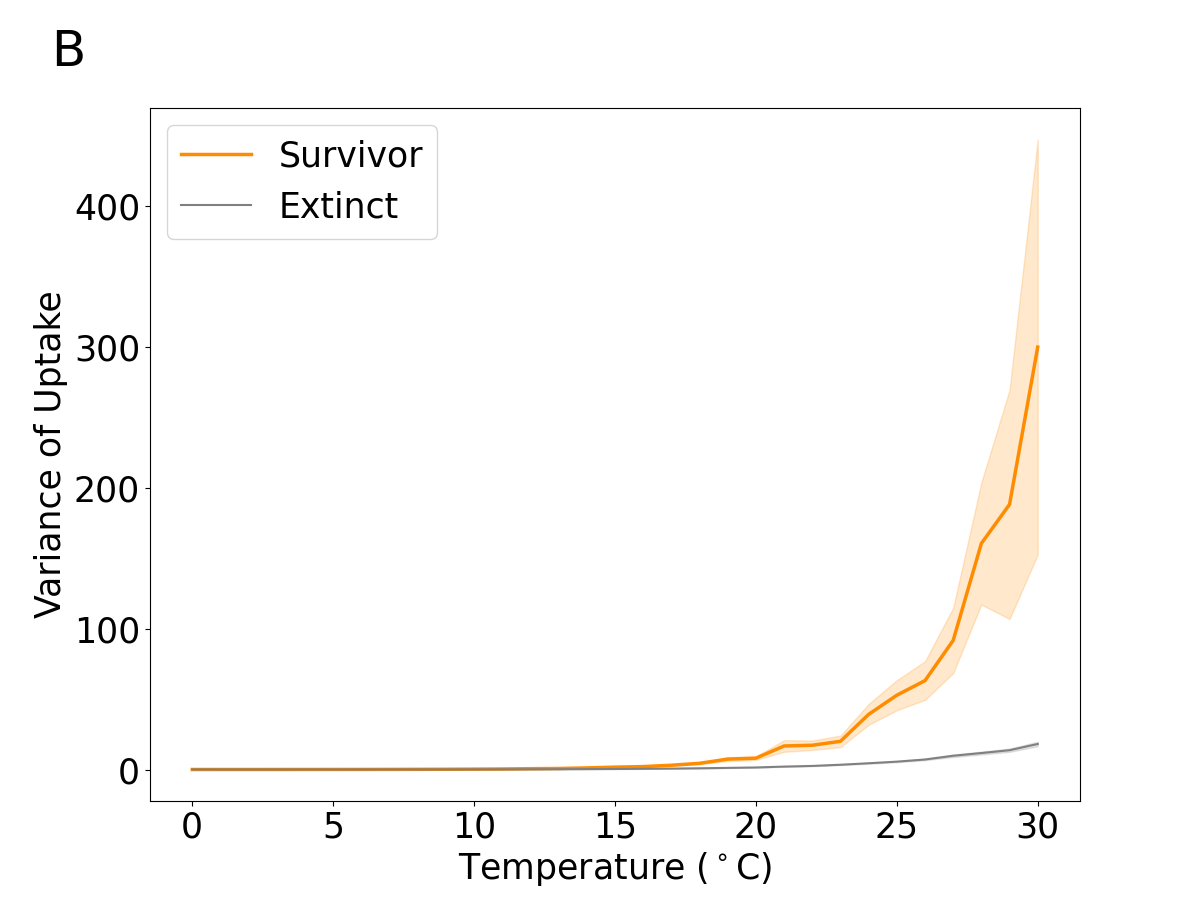
\includegraphics[scale=0.27]{./Figures/VarU.png}
    \end{tabular}
    \caption{\textbf{The selection on pairwise species interactions at different temperatures.} A: Resource overlap and interspecies facilitation ability of survivors and extinct species across temperatures. Plotted with 95\% CI bands of facilitation and competition values for survivors and extinct species at each temperature. B: The average variance of uptake rates among resources of each survivor species and each extinct species at different temperatures, with 95\% CI bands of these values at each temperature. High values depict that the species have distinctively higher uptake of few resources and distinctively lower uptake of the rest.}
    \label{fig:cf}
\end{figure}

Next, to obtain deeper insights into the mechanisms driving the changes in species diversity with temperature, I test whether a more facilitative environment can mitigate the diversity loss at higher temperatures by increasing the leakage fraction of resources (Section \ref{sec:lf} in Supplementary Information). I find that leakage does not significantly impact the pattern of decline in species richness with increasing temperature. I also find that facilitation is favored at low temperatures for high leakage communities, at high temperatures for low leakage communities. And at a high leakage fraction of $l=0.7$, species richness was in fact lower than in less facilitative environments. The figure demonstrations are in Figure \ref{fig:lf} in Supplementary Information. 

\section{Discussion}

I have investigated the richness of model microbial communities assembled at different temperatures, focusing on the role of metabolic strategies and thermal physiology in species sorting and coexistence. With a metabolically constrained mathematical model, I find that heterotrophic microbial community richness typically declines within an operational mesophilic temperature range. 

\subsection{Emergent community CUE as a result of species sorting}

Since the thermal sensitivities for physiology traits ($E_{a_U}$ and $E_{a_R}$) are different among species, meaning that the magnitude of their increases with temperature differ among species. These differences are enlarged with increasing temperature as species' trait values increase exponentially with temperature following equation \ref{eq:U+R}. This leads to the increasing variation of intrinsic CUE values, however species sorting at higher temperatures resulted in a smaller non-random subset of CUE values, corresponding to the increasing magnitude of competitive exclusion, that only species with the highest CUE (lowest $S^*$) survive. 

Besides the numeric link between species $E_{a_{CUE}}$ and $S^*$, that competitive exclusion results in the elimination of low $E_{a_{CUE}}$(i.e. higher $S^*$) species. The higher species $E_{a_{CUE}}$ in communities assembled at higher tmperatures can also be explained by the selection on higher intrinsic CUE. To achieve this high intrinsic CUE values for succeeding in resource competitions at higher temperatures, the differences between species thermal sensitivities in resource uptake and respiration rates ($E_{a_U} - E_{a_R}$) need to be sufficiently large. As shown in Equation \ref{eq:EaCUE}, species $E_{a_{CUE}}$ represents the metabolic strategies of species thermal physiologies by describing these differences in thermal sensitivities of metabolic rates. Therefore, species with low $E_{a_{CUE}}$ are more likely to be eliminated during species sorting at high temperatures, as shown in Figure \ref{fig:EaCUE}B. This is especially true for species with a negative $E_{a_{CUE}}$. As for these species, the respiratory carbon loss rate exceeds carbon uptake rate with increasing temperature, meaning that higher temperatures are unfavorable for their growth. These results show that even if the thermal sensitivities of resource consumption and maintenance respiration vary independently for each individual species \citep{pold2020carbon}, the emergent community-level CUE (as well as $E_{a_{CUE}}$) would still be increasing with temperature as a result of species sorting.

\subsection{The contribution of species interactions to coexistence at different temperatures}

At low temperatures, especially at reference temperatures, the metabolic rates of species are relatively low, and the resource limitation is relatively released. As shown in Figure \ref{eq:EaCUE}A, the effective competition for resources is relatively lower among species. Under this scenario, the external resource supply combined with the averagely distributed cross-feeding products can support more species with higher overlapping resource requirements. 

As temperature increases, the resources are becoming increasingly limited since the external resource supply is temperature independent and constant across temperature range. As the strength of effective competition increases, facilitation is generally favoured for supporting the growth and coexistence of species \citep{seth2014nutrient, pascual2020metabolically} as shown in Figure \ref{fig:cf}A, since facilitation activities engineer the surrounding resource environment by producing metabolic by-products as secondary carbon resources. To coexist in this increasing limitation on carbon resources, species would need to have different resource uptake strategies to reduces the overlaps of resource uptake with each other \citep{chesson2000mechanisms}. Therefore, resource partitioning increased with rising temperature. Specialists species who specifies at fewer resources (with higher uptake rates on few resources and lower uptake rates on others, Figure \ref{fig:cf}B) are favored at high temperatures. 

Based on the leakage-transformation matrix (Figure \ref{fig:schematic}), the metabolic by-products are secreted averagely across resource types down the reaction gradient. Since specialists species have distinctively high uptake in few resources and distinctively lower in the rest, the overlap of their resources uptake with these evenly generated metabolites is lowered. Therefore, some of the metabolites secreted by another species would be redundant for their resources requirement. 

However, even though facilitation is generally beneficial for microbial communities, high facilitation may be detrimental for species diversity. This is because high leakage means lower resource utilization efficiency (lower CUE), leaving insufficient resources for cell growth (Equation \ref{eq:CUE_i}). In this scenario species require an even higher resource uptake to achieve the CUE for succeeding in resource competition. This leads to more intense resource limitation, and higher strength of effective competition among species. Secondly, high by-product secretion reduces the concentration of species' preferable resources, which is especially detrimental when the resources environment is highly competitive. 

Therefore, combining with the inefficiency in cross-feeding production at high temperatures, relatively lower facilitation is again starting to be favored at higher temperatures, where resources are relatively more limited. In addition, this result suggests that facilitation can only support species coexistence and mitigate diversity loss to an extend, beyond that , facilitation is in fact detrimental for coexistence. The balance and dominance of the benefits and detriments of facilitation combined determines either relatively high or low facilitation is favored for species survival and maintaining coexistence at each temperature. The trade-off between can be clearly seen at medium temperatures around 10 - 15 \textdegree C (Figure \ref{fig:cf}). 

\subsection{Empirical relevance of CUE and richness patterns}

\subsubsection{Empirical relevance of the emergent community CUE}

In this study, with a low CUE value of 0.22 at 0 \textdegree C \citep{smith2020systematic}, the highest value of average community CUE is predicted to be about 0.57 at 30 \textdegree C. This range of CUE mostly lies within the results of previous empirical studies of approximately 0.24 to 0.77 \citep{geyer2016microbial}, and metabolic modeling prediction which is a larger range of bacterial CUE from 0.22 to 0.98 \citep{saifuddin2019microbial}. Previous studies on the temperature response of community CUE reported different trends of increasing \citep{sinsabaugh2016stoichiometry}, decreasing \citep{qiao2019global, steinweg2008patterns} or no response with temperature \citep{oquist2017effect}. 

Since here I have only considered community CUE as the result of species sorting, other factors may as well influence the temperature dependence pattern of CUE. Firstly, I calculated CUE as the fraction of resource uptake allocated to growth, whereas different measurements and calculation methods could lead to different results in CUE \citep{geyer2019clarifying}. Secondly, other abiotic environmental factors such as nutrient limitation could constrain the thermal sensitivities of species resource uptake, resulting in lower CUE values at high temperature. For example, species resource uptake rates can be constrained by the rate of carbon fixation in surrounding environment, the thermal sensitivity of which is lower than species respiration \citep{allen2005linking, sinsabaugh2017plant}. Finally, species may exhibit physiological thermal adaptations \citep{sinsabaugh2016stoichiometry, bradford2013thermal, kontopoulos2020adaptive} and trade-offs such as between CUE and growth rates \citep{roller2016exploiting} or resource uptake rates \citep{allison2014modeling} on genomics level. Though these genomics characteristics might not be as definitive as physiological traits while considering the emergent community-level CUE \citep{pold2020carbon}. 

$E_{a_{CUE}}$ is suggested as a better subject for comparison when considering the temperature response of microbial CUE across environmental gradients, to disregard the impacts of nutrients limitation in natural conditions\citep{pold2020carbon}. Therefore, I conclude that species resource utilization ability increases with temperature since community $E_{a_{CUE}}$ increases with temperature within specie OTR as the result of this study.

\subsubsection{Empirical relevance of the emergent community richness}

After decades of conflicting reports about patterns of species richness along temperature gradients \citep{hendershot2017consistently}, a global study conducted by Earth Microbiome Project (EMP) \citep{thompson2017communal} revealed a unimodal pattern of global microbial diversity with temperature, where maximum microbial diversity appeared at intermediate temperature values around 10 \textdegree C. 

\cite{marsland2020minimal} used the Microbial Consumer Resource Model (MiCRM) to interpret this result. The microbial community model used in this study (Equation \ref{eq:community}) is based on the MiCRM. They successfully reproduced the unimodal shape by adding increasing randomly generated values to maintenance cost for simulations on temperatures away from the observed optimum temperature of richness (10 \textdegree C), deeming these temperatures as harsher environments. This idea stems from the expectation that microbes require increased resource consumption to satisfy the increased energy demands for survival in harsh environments \citep{hoehler2013microbial}. However, there is no ecological or evolutionary background supporting 10 \textdegree C to be the optimum temperature for microbial growth or coexistence in majority. Therefore, simply assuming temperatures away from 10 \textdegree C as harsh environments seems less adequate comparing to the approach of constraining the model with temperature dependent traits in this study. 

The deviation of my results from EMP dataset possibly includes that: First of all, I am neglecting the inactivation of organisms’ enzymes at low temperatures \citep{nedwell1999effect, schoolfield1981non}. Since the decline of traits at low temperatures varies for different enzymes \citep{sharpe1977reaction}, species would again exhibit varying $CUE$ and $E_{a_{CUE}}$ values at low temperatures. If this is considered, species richness would possibly drop at these low temperatures as a result of species sorting. Secondly, in this study, I am only modelling the communities of mesophiles, neglecting the communities of psychrophiles whose metabolic rates normally peak at about 15 \textdegree C or lower \cite{moyer2007psychrophiles}. 

\subsection{Caveats and future directions}

The prevalent meta-omics approaches alone cannot fully or directly map the highly complex network of interspecies and metabolic interactions. Therefore, the construction of such networks and the the complete understanding of microbial communities cannot be achieved solely depending on pure empirical (laboratory or field) approaches. Mathematical modelling offers a complementary way to understand these complex systems mechanistically by controlling for confounding factors \citep{hanemaaijer2015systems, marsland2020minimal}, such as disentangling the impacts by various environmental factors and differentiating the effects of species interactions. 

Here, I focused singularly on the impacts of environmental temperature and the species interactions relevant to resource utilization. Base on my study, further work on the temperature dependence of species richness and CUE could include: 

1) Further understanding on this microbial community system. Firstly, the equilibrium states of the system can be numerically interpreted further, especially extending into the mechanisms of the coexistence of multispecies and multi-resources at equilibrium. Secondly, for further understanding of the impacts of facilitation on species coexistence at different temperatures, a variation in species metabolic products secretion can be considered \citep{grosskopf2016microbial}. In addition, the thermodynamic constrains on metabolic products transformation can also be considered. 

2) Model comparison. The thermal response constraints can be implemented into different ecological models to compare simulation results. 

3) Combination with empirical studies. Laboratory analysis can be conducted in addition to this modelling approach. This can provide results for the richness and CUE patterns of the communities assembled at different temperatures under controlled environments, which is useful for model validation and further adjusting mathematical models to "real-life" scenarios. 

4) Considering additional elements. Firstly, psychrophiles communities can be introduced to relate to a wider ecological content. Secondly, the trade-offs between metabolic traits could be considered for adaptation into this model. Finally, other environmental impacts such as pH and moisture \citep{manzoni2012environmental, fierer2009global} and biotic factors such as toxin excretion \citep{stempler2017interspecies} can also be added into this model framework. By adding these factors, a more complete understanding on the patterns and mechanisms under microbial diversity along global gradients can be obtained.


\section{Conclusion}

In conclusion, using a novel mathematical model of microbial community assembly dynamics, I have demonstrated a negative correlation between species richness and community assembly temperatures. Species sorting during community assembly is the major driver for the decline of richness along temperature gradient, driven by selection on species' metabolic strategies of thermal physiologies. As the result of species sorting, community CUE and $E_{a_{CUE}}$ increased with rising temperature, suggesting higher resource utilization ability in communities assembled at higher temperatures. Resource partitioning increased with temperature and specialists favored at higher temperatures. Facilitation mediated diversity loss to an extend, however high facilitation become less effective and relatively less supportive for species coexistence at high temperatures. To the best of my knowledge, this is the first theoretical study on the effect of temperature on diversity and its link with the emergent CUE of complex microbial communities. This study provides new mechanistic insights into geographical patterns of microbial diversity and their relation to global carbon cycling. 

\section*{Code Availability}
\addcontentsline{toc}{section}{Code Availability}

The python code for model simulation and analysis in this study is availible at the \href{https://github.com/DaniDuan/CMEEProject}{\color{blue}{\underline{CMEEProject}}} repository.

\section*{Acknowledgement}
\addcontentsline{toc}{section}{Acknowledgement}

I would like to express my greatest gratitude to Dr. Samraat Pawar for all his support and supervision throughout the entire project, even after his sabbatical started. I'm also sincerely grateful for all the inspiring ideas and thoughts Tom Clegg (PhD candidate) and Dr. Tom Smith provided throughout my project. And thank all three of them for providing feedback on my drafting thesis. In the end I would like to thank everyone who has emotionally supported me over this academic year, include but not limited to my parents, my friends and my amazing boyfriend Sibo Zhang. 

\bibliographystyle{agsm}
\bibliography{thesis}
\clearpage


\begin{document}
\renewcommand{\thefigure}{SI.\arabic{figure}}
\setcounter{figure}{0}

\section*{Supplementary Information}\label{sec:SI}

\addcontentsline{toc}{section}{Supplementary Information}
\addtocontents{toc}{\setcounter{tocdepth}{-10}}
\renewcommand{\thesubsection}{SI.\arabic{subsection}}
\setcounter{subsection}{0}

\subsection{Vectorized model and abundance dynamics in community simulation}

The consumer and resource dynamics in the simulation is calculated using the vectorized version of equations 1 \& 2 for computing efficiency: 

\begin{align*}
&\frac{d\mathbf{C}}{dt} = diag(\mathbf{C}) \circ ((1-l) \mathbf{U} \cdot \mathbf{S} - \mathbf{R})\\
&\frac{d\mathbf{S}}{dt} = \boldsymbol{\rho} - diag(\mathbf{S})\cdot \mathbf{U}^T \cdot \mathbf{C} + (\mathbf{U} \cdot diag(\mathbf{S}) \cdot \mathbf{l})^T \cdot \mathbf{C}
\end{align*}
In these equations, $\mathbf{C}$ and $\mathbf{S}$ are single row matrices of consumer and resource concentration at each time point. $\mathbf{U}$ is the N $\times$ M matrix of species uptake rate, $\mathbf{R}$ is the single row matrix of species respiration rate with the length of N. $\mathbf{l}$ is the M $\times$ M leakage matrix for M resources, and l is the set leakage fraction of resources. "$\circ$" denotes the element wise product of two matrices, "$\cdot$" represents matrix multiplication, and "T" is the transpose of matrix. $diag(\mathbf{C})$ is setting the consumer concentration at each time point onto the diagonal of N $\times$ N matix with the rest of the elements as 0. $diag(\mathbf{S})$ is setting the resource concentration at each time point onto the diagonal of M $\times$ M matix with the rest of the elements as 0, which notation makes the calculation equivalent to calculating row-wise products of $\mathbf{U}$ and $\mathbf{S}$. 

The plot below (Figure \ref{fig:example}) shows an example of the abundance dynamics of $N = 100$ species of heterotrophic bacterial consumers competing for $M = 50$ resource types at $T_{ref}$ ($T = 0$ \textdegree C). The figure is plotted with 1000 time steps (which is before the system reaches steady state), however it has already shown that a large number of species' biomass drop to extinction shortly after the simulation started, while none of the resources went extinct.

\begin{figure}[H]
    \centering
    \begin{tabular}{c@{}c@{}}
    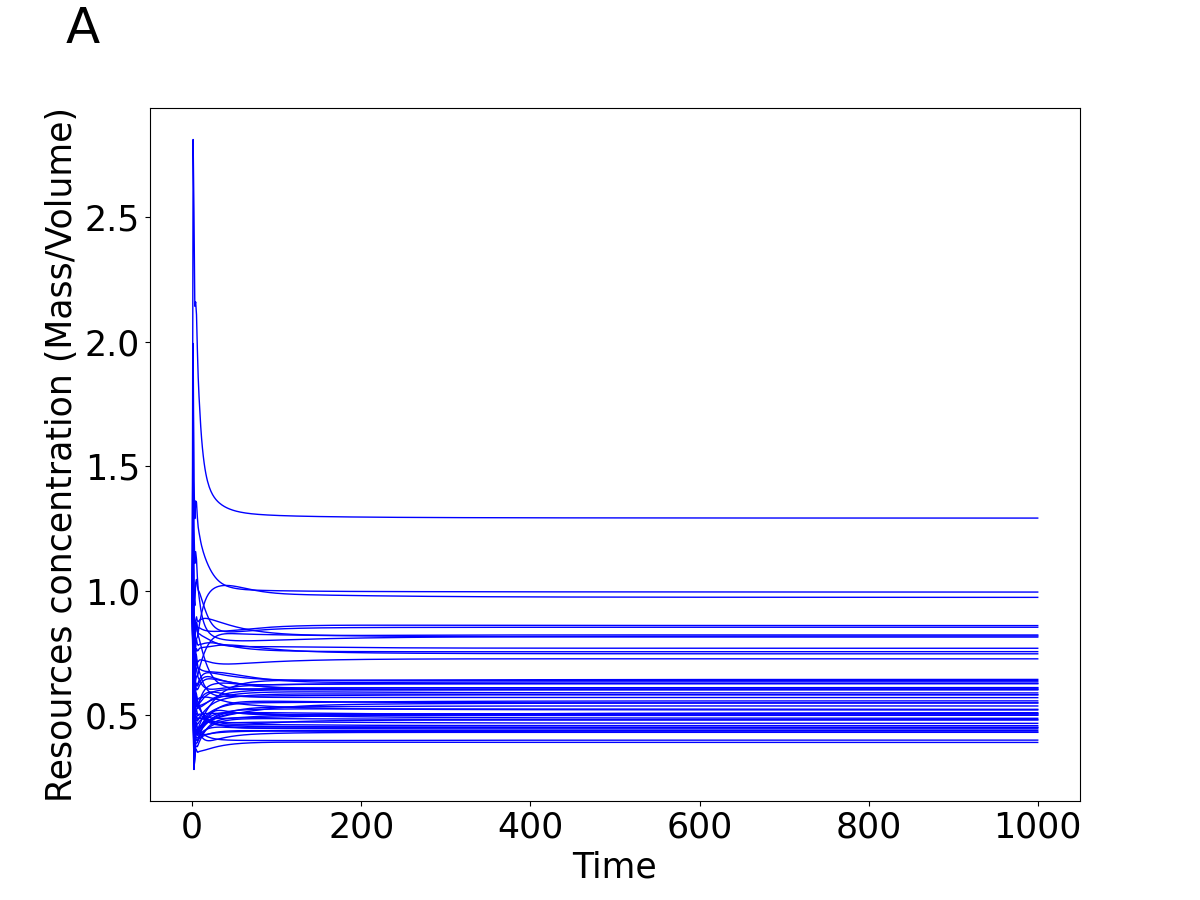
\includegraphics[scale=0.27]{./Figures/resource_con_example.png}
    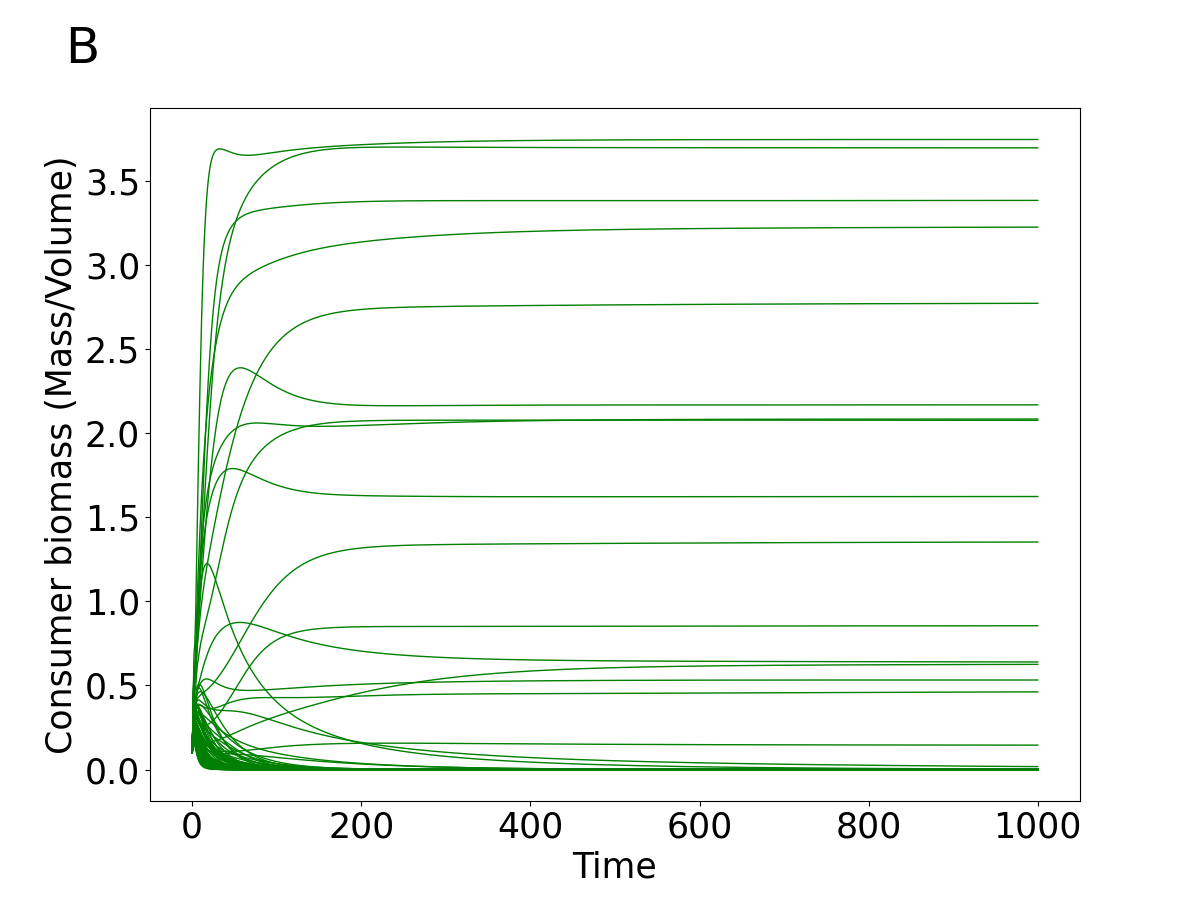
\includegraphics[scale=0.27]{./Figures/consumer_con_example.png}
    \end{tabular}
    \caption{\textbf{Example plots showing the resources concentration and consumers biomass dynamics of one assembly.} Plotted with 1000 time steps at reference temperature, $N = 100$ consumers competiting for $M = 50$ resources.}
    \label{fig:example}
\end{figure}

\subsection{TPCs of metabolic rates}

\begin{figure}[H]
    \centering
    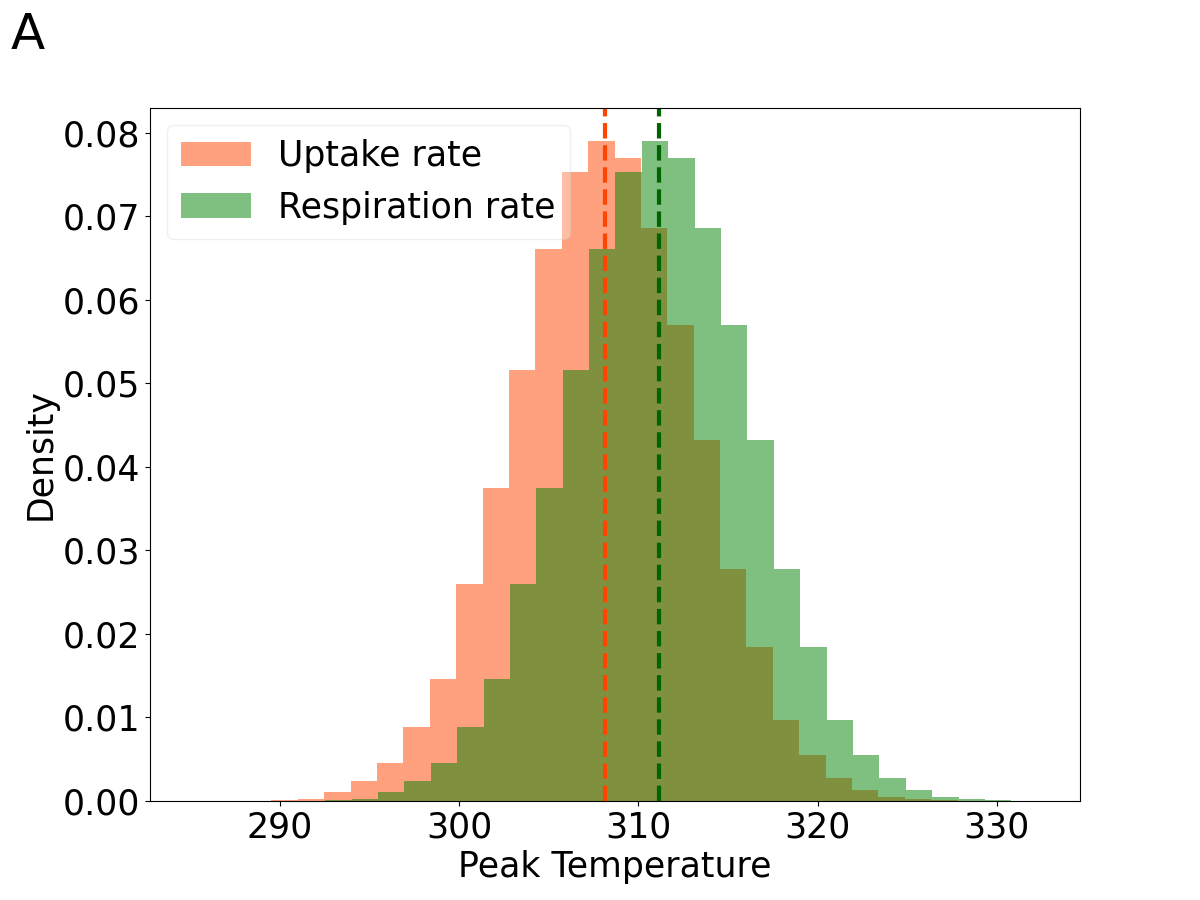
\includegraphics[scale=0.27]{./Figures/SI_UR.png}
    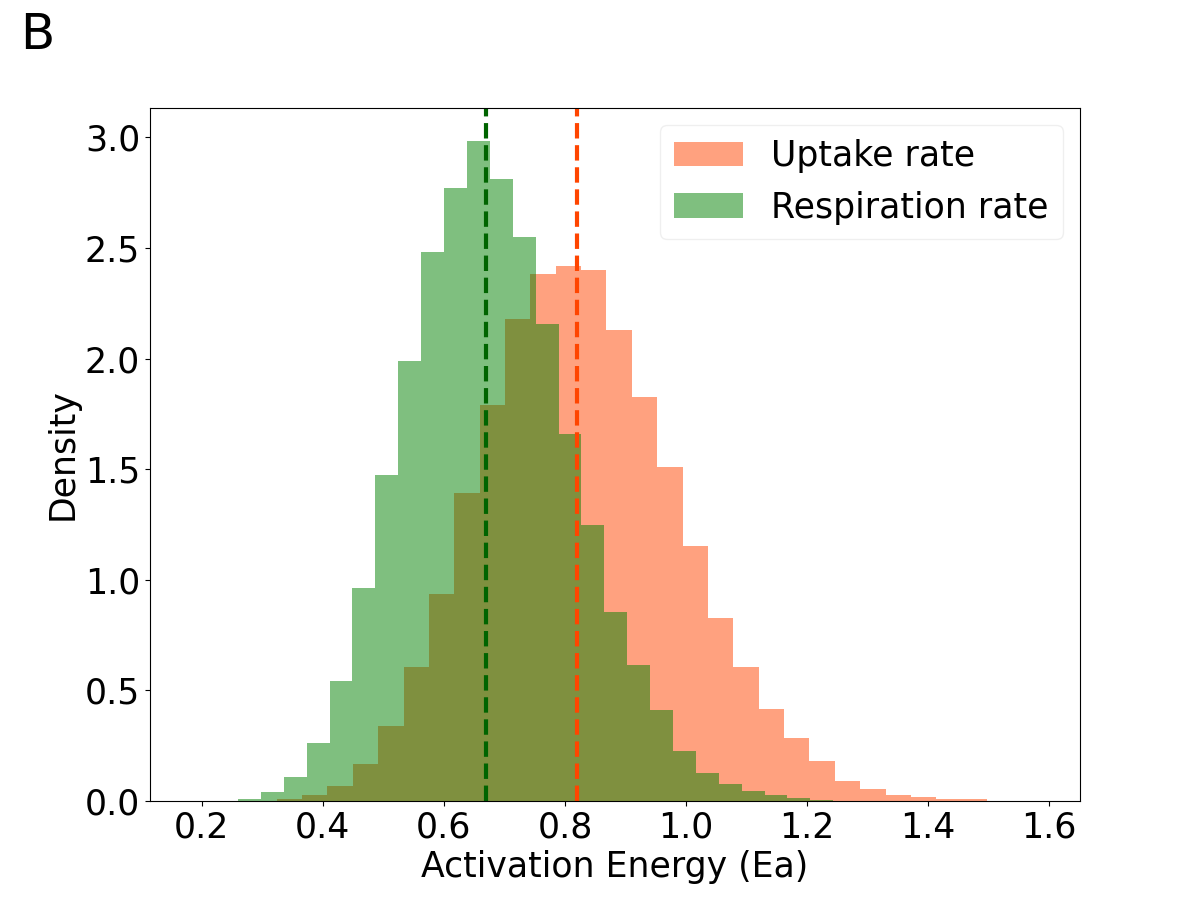
\includegraphics[scale=0.27]{./Figures/SI_UR_1.png}
    \caption{\textbf{Histogram of randomly sampled $T_{pk}$ and $E_a$ values for uptake and respiration rates.} A: $T_{pk_U}$ was sampled from a normal distribution with mean value at 308.15 $K$, and $T_{pk_R} = T_{pk_U} + 3$ to make sure species respiration always peak higher than uptake. The dotted lines in the middle depict the mean values of uptake (orange) and respiration (green) rates peak temperatures. B: $E_a$ values are sampled from beta distributions ($\alpha = 15$) with median values of 0.82 $eV$ and 0.67 $eV$ for uptake and respiration.The dotted lines in the middle depict the median values of the thermal sensitivities of uptake (orange) and respiration (green) rates. The densities are shown with 50000 randomly generated values. }
    \label{fig:SI_UR}
\end{figure}

\begin{figure}[H]
    \centering
    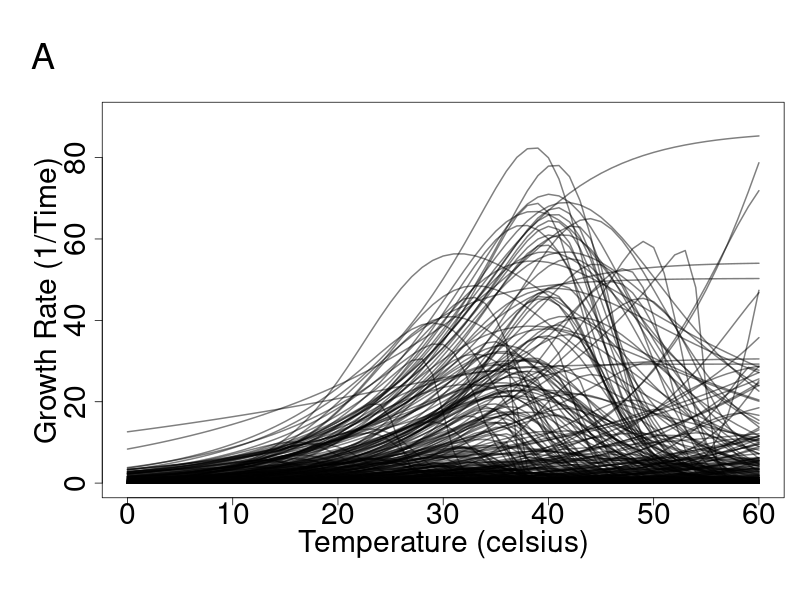
\includegraphics[scale=0.3]{./Figures/BioTrait_growth.png} \\
    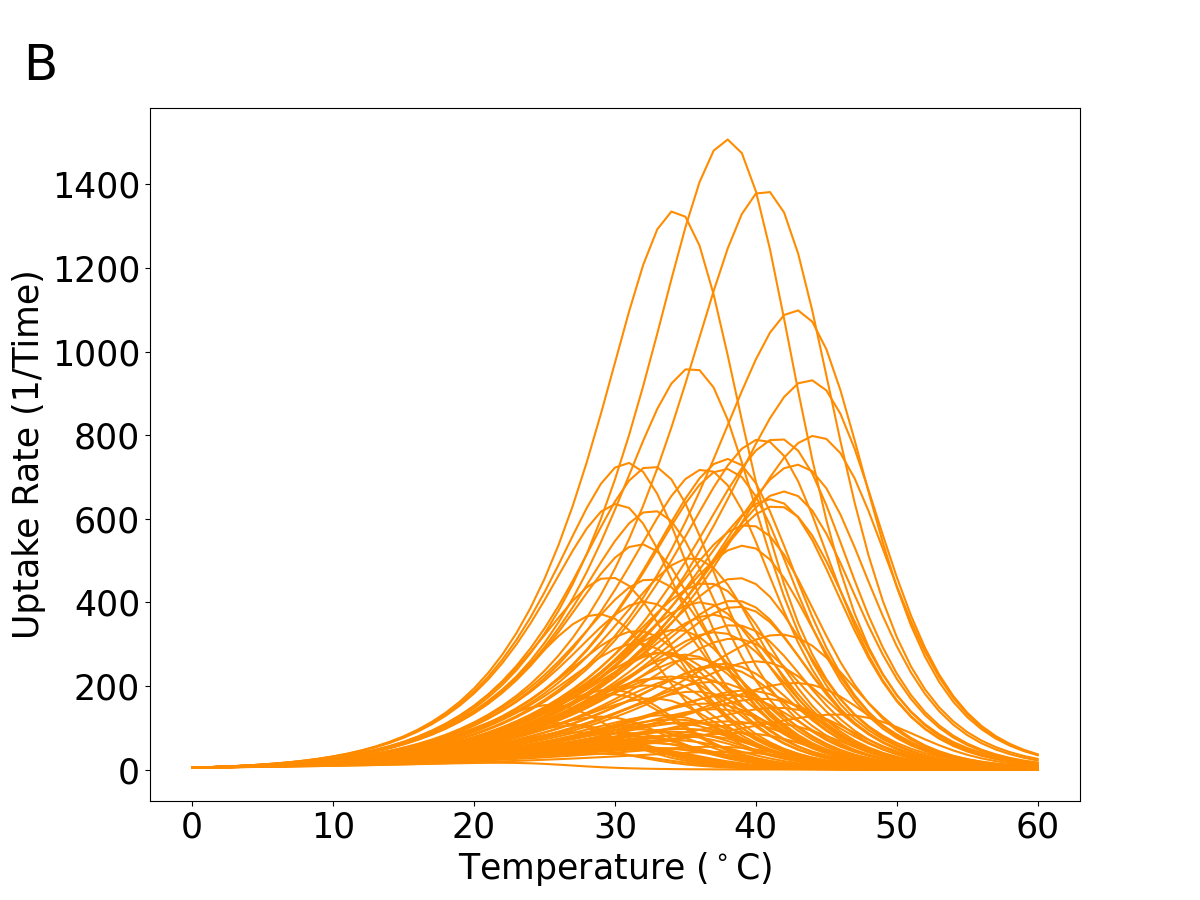
\includegraphics[scale=0.27]{./Figures/simulated_uptake_rate.png}
    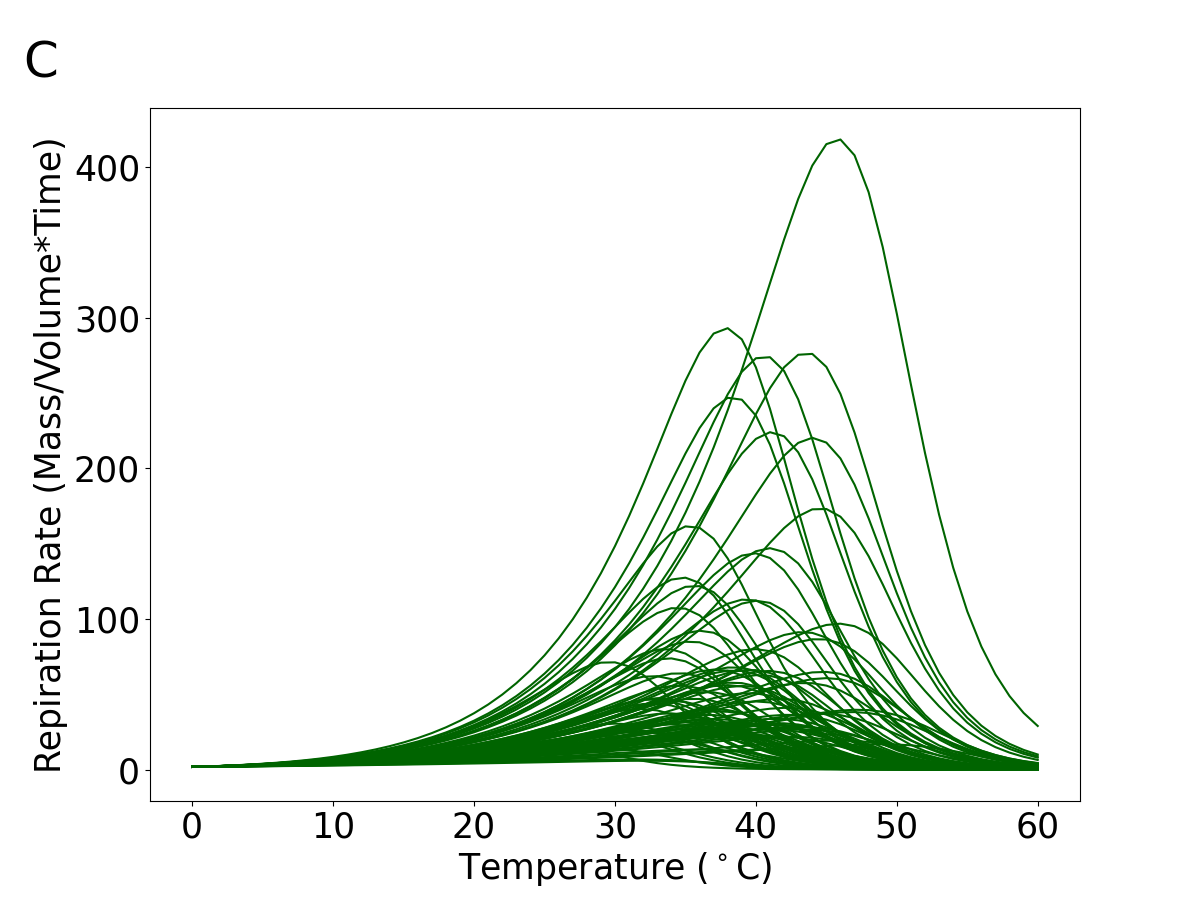
\includegraphics[scale=0.27]{./Figures/simulated_res_rate.png}
    \caption{\textbf{The temperature dependence curves of species growth, uptake and respiration rates.} A: The temperature performance curves of bacterial growth rates generated by fitting the modified Schoolfield temperature dependence equation, using the global data set collected and standardized by \cite{smith2019community}. B \& C: Example of a randomly generated set of temperature dependency curves for consumer uptake ($U_i$) and respiration ($R_i$) rates ($N$ = 100). Assuming resource uptake is majorly allocated to growth and respiration: $U \approx R + \mu$.}
    \label{fig:G}
\end{figure}

\subsection{Derivation of equations linking competitive exclusion and metabolic strategies}\label{sec:S+CUE}

The equilibrium resource concentration requirement for the $i^{th}$ species ($S^*$) can be calculated by rearranging equation \ref{eq:community} with $dC_i/dt = 0$, getting:

\begin{equation*}\label{eq:S*}
S^*_i = \frac{R_i}{U_i(1-l)}
\end{equation*}
The Arrhenius equation can be implanted here for species growing in OTR:

\begin{equation*}
S^*_i = \frac{R_0 e^{\frac{-Ea_R}{k}\cdot\left(\frac{1}{T} - \frac{1}{T_{ref}}\right)}}{U_0 e^{\frac{-Ea_U}{k}\cdot\left(\frac{1}{T} - \frac{1}{T_{ref}}\right)} (1-l)}
\end{equation*}
Take a log form of the equation, and set $\Delta T = \frac{1}{k}\left(\frac{1}{T} - \frac{1}{T_{ref}}\right) $:

\begin{equation*}
lnS^*_i = lnR_0 - ln(1-l)U_0 + (Ea_U - Ea_R) \Delta T
\end{equation*}

In this equation, since $R_0$ and $U_0$ values do not differ between species, the comparison of $S^*$ values lies completely in the differences between $Ea_U$ and $Ea_R$. Since at temperatures higher than reference temperature, the $\Delta T$ value is negative, so the species with higher $Ea_U - Ea_R$ value will have lower $S^*$, therefore winning the competition. 

In this case, the resource requirements for survival can be linked to species intrinsic CUE values (equation \ref{eq:CUE_i}), as:
\begin{equation}\label{eq:S_CUE}
CUE_i = (1 - S^*_i) (1-l)
\end{equation}
Therefore, the advantage of lower resource requirement in resource competition is related to the selection on higher intrinsic CUE values.

Since winner species with higher fitness (lower $S^*$) has higher $Ea_U - Ea_R$ value, these species also have higher $E_{a_{CUE}}$ (equation \ref{eq:EaCUE}). The relationship between species fitness and $E_{a_{CUE}}$ can also be shown in equation as:
\begin{equation}\label{eq:S_Ea}
lnS^*_i = lnR_0 - ln(1-l)U_0 + \frac{U_0(1-l) - R_0}{R_0}E_{a_{CUE}}\Delta T
\end{equation}

\begin{figure}[H]
    \centering
    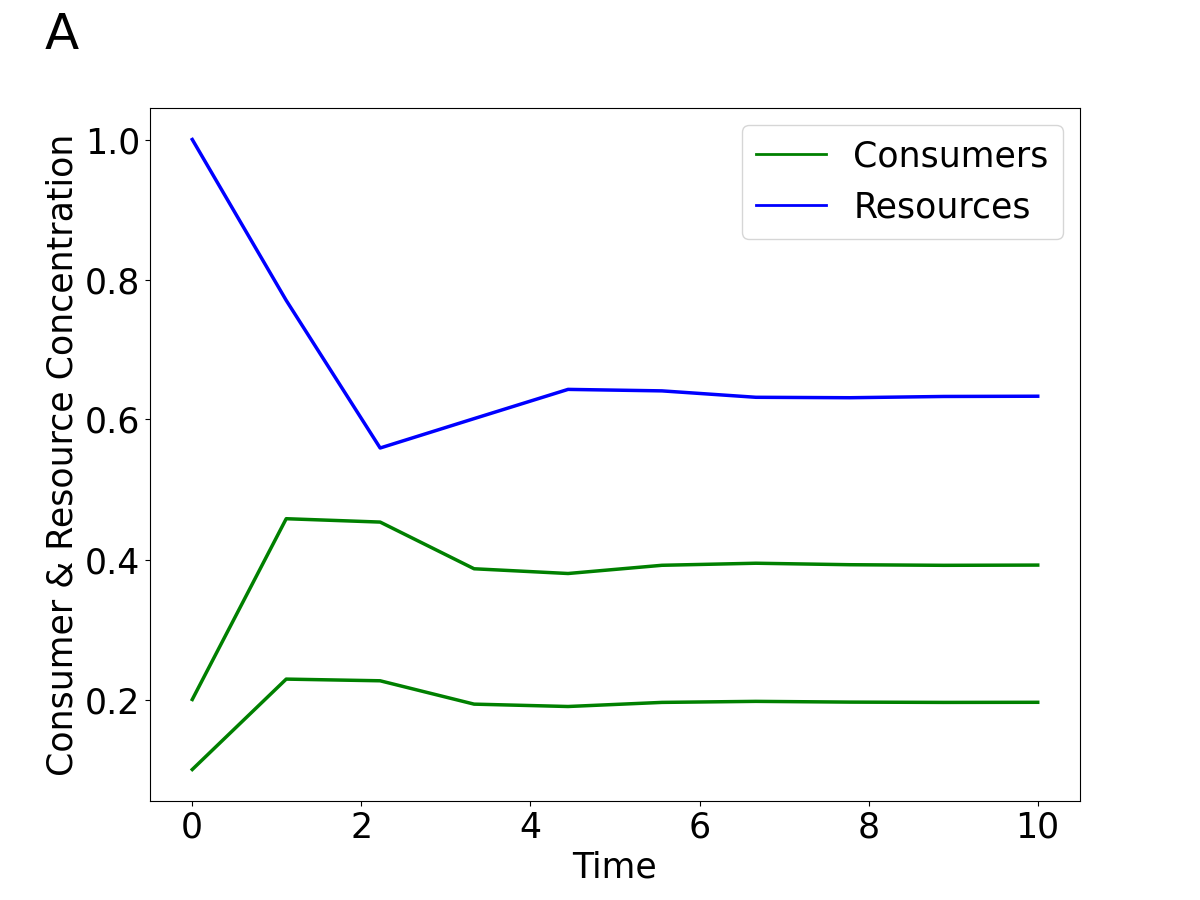
\includegraphics[scale=0.27]{./Figures/2_consumer_Tref.png}
    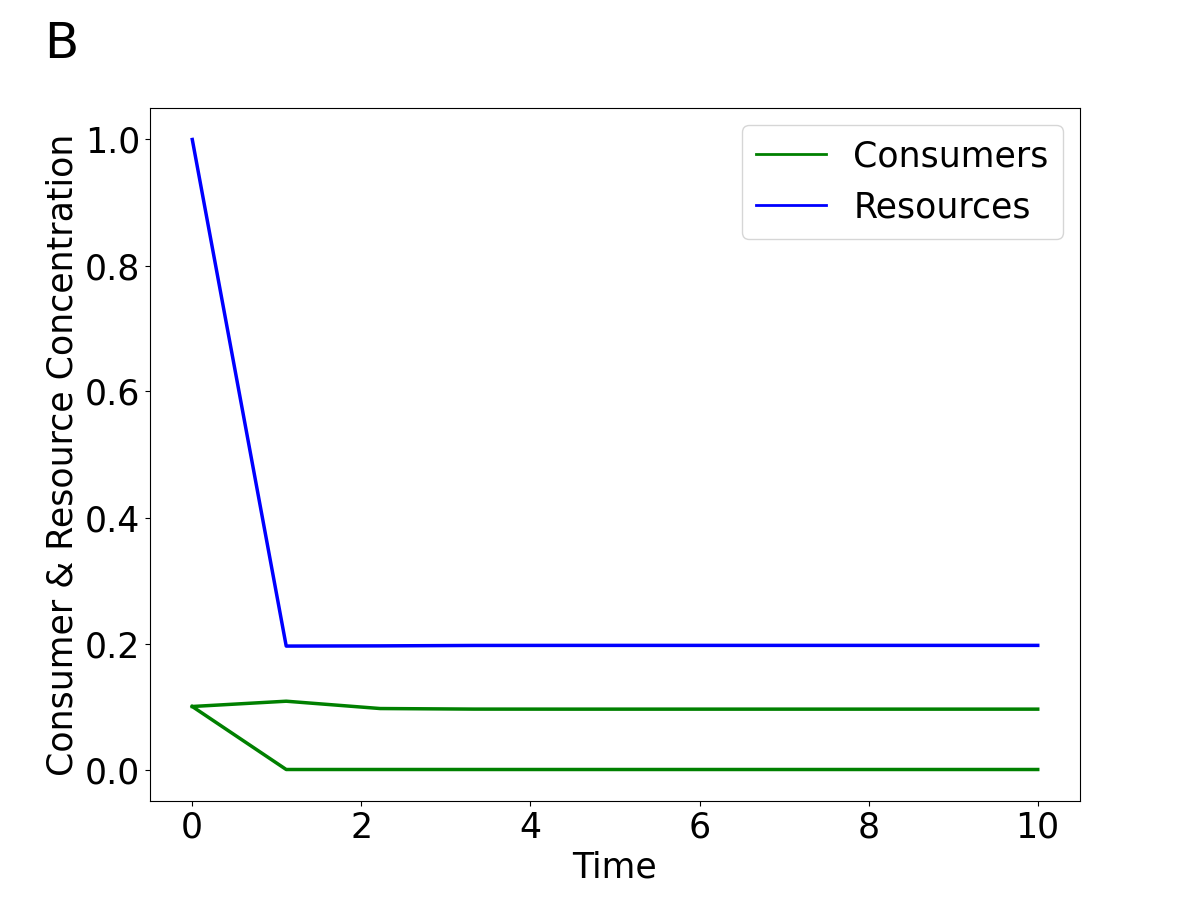
\includegraphics[scale=0.27]{./Figures/2_consumer_25C.png}
    \caption{\textbf{Example plots of the consumers and resource concentration dynamics of two species competing for one resource at reference temperature and at 25 \textdegree C.} A: At reference temperature, both species have the same $S^*$ therefore have the same growth rate regardless of their initial biomass. B: At temperatures higher than reference temperature, species have different $S^*$, competitive exclusion results in only one survivor.} 
    \label{fig:2_example}
\end{figure}

\subsection{Type II functional response}

For the robustness of qualitative results, I implemented Type II functional response (Monod function) into resources uptake. Note the resources uptake rates here has the unit of Mass/Volume*Time, which contains the concentration of species uptake at each time step. The uptake rate of $M^{th}$ resource by $i^{th}$ species: 
\begin{equation*}
    U_{m_{ij}} = U_{ij}\cdot\frac{S_j}{K+S_j}
\end{equation*}
K here is the half saturation constant of the $j^{th}$ resource. As shown in Figure \ref{fig:TypeII}B, implementing the Type II functional response into simulations does not significantly change the species richness pattern with assembly temperatures. 

\begin{figure}[H]
    \centering
    \begin{tabular}{c@{}c@{}}
    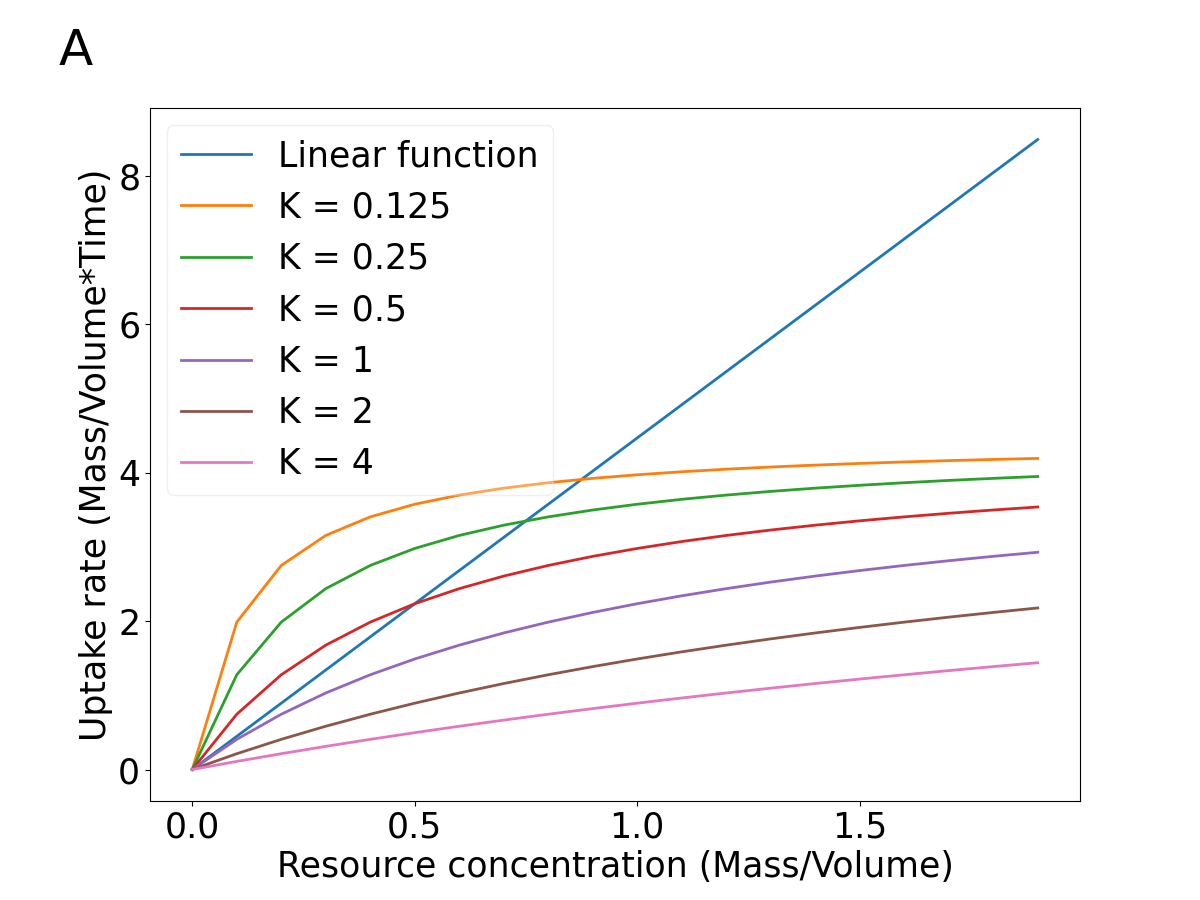
\includegraphics[scale=0.27]{./Figures/K.png}
    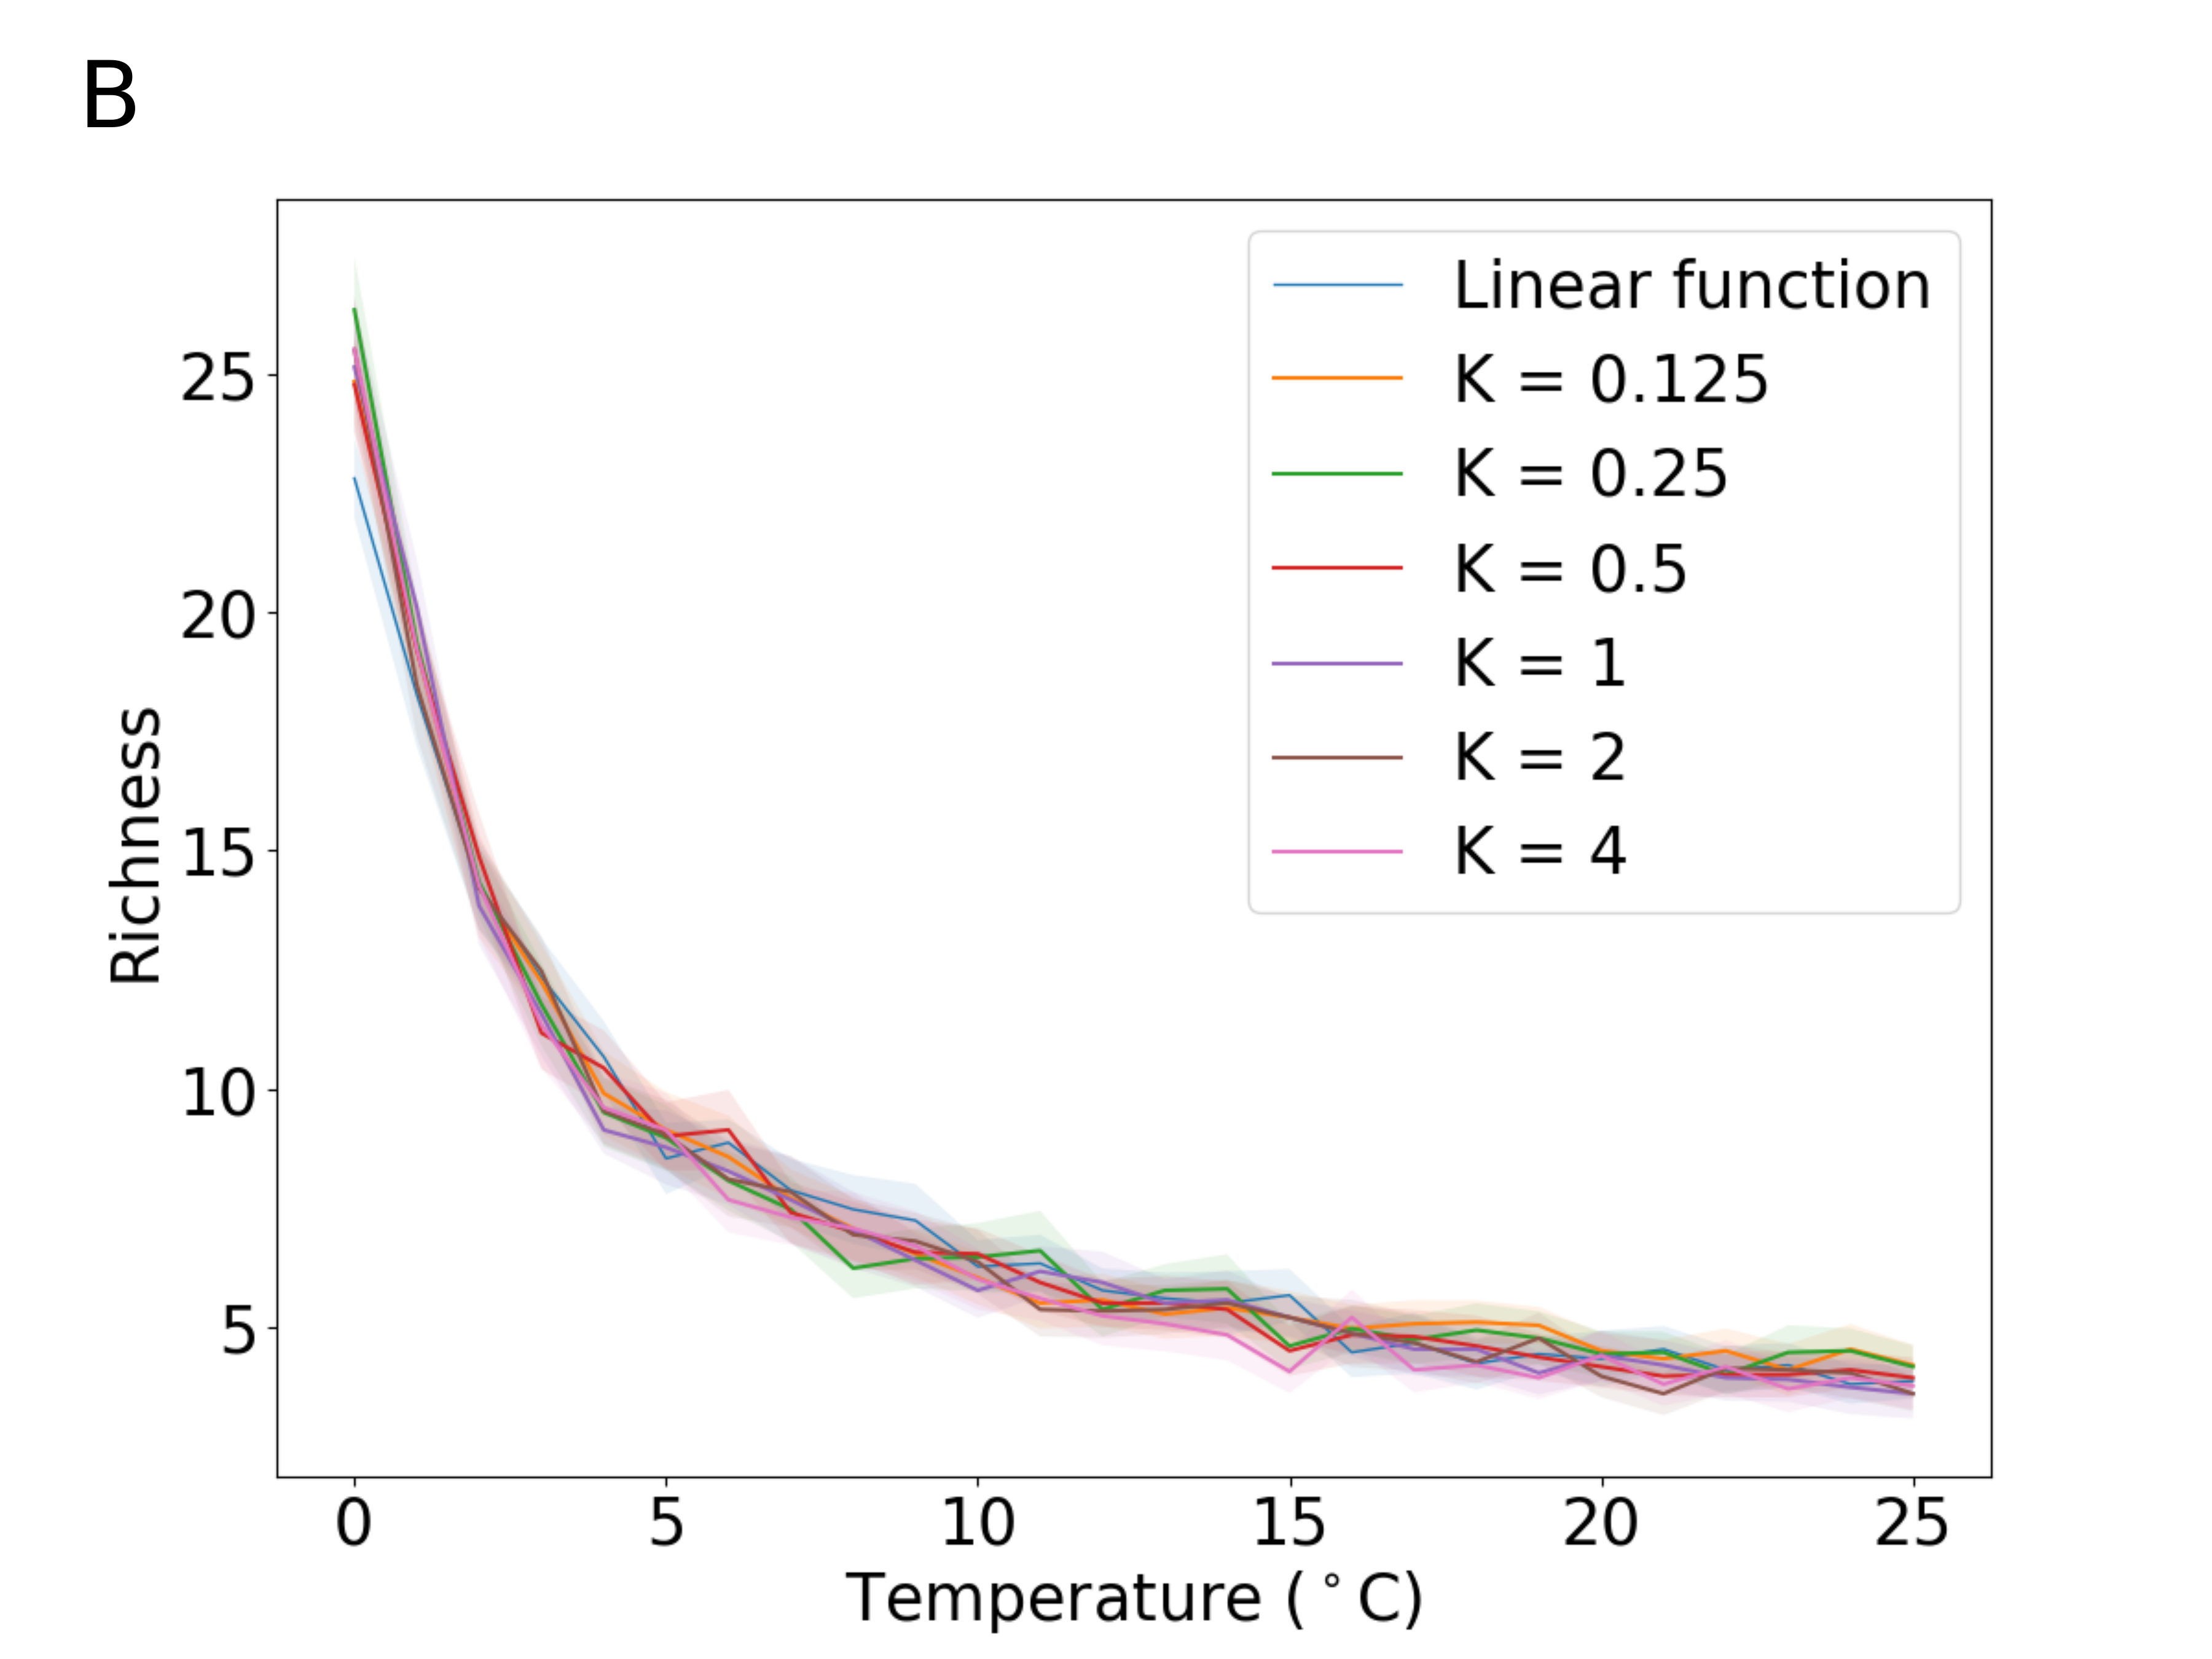
\includegraphics[scale=0.27]{./Figures/K_rich.png}
    \end{tabular}
    \hfill
    \begin{tabular}{c@{}c@{}}
    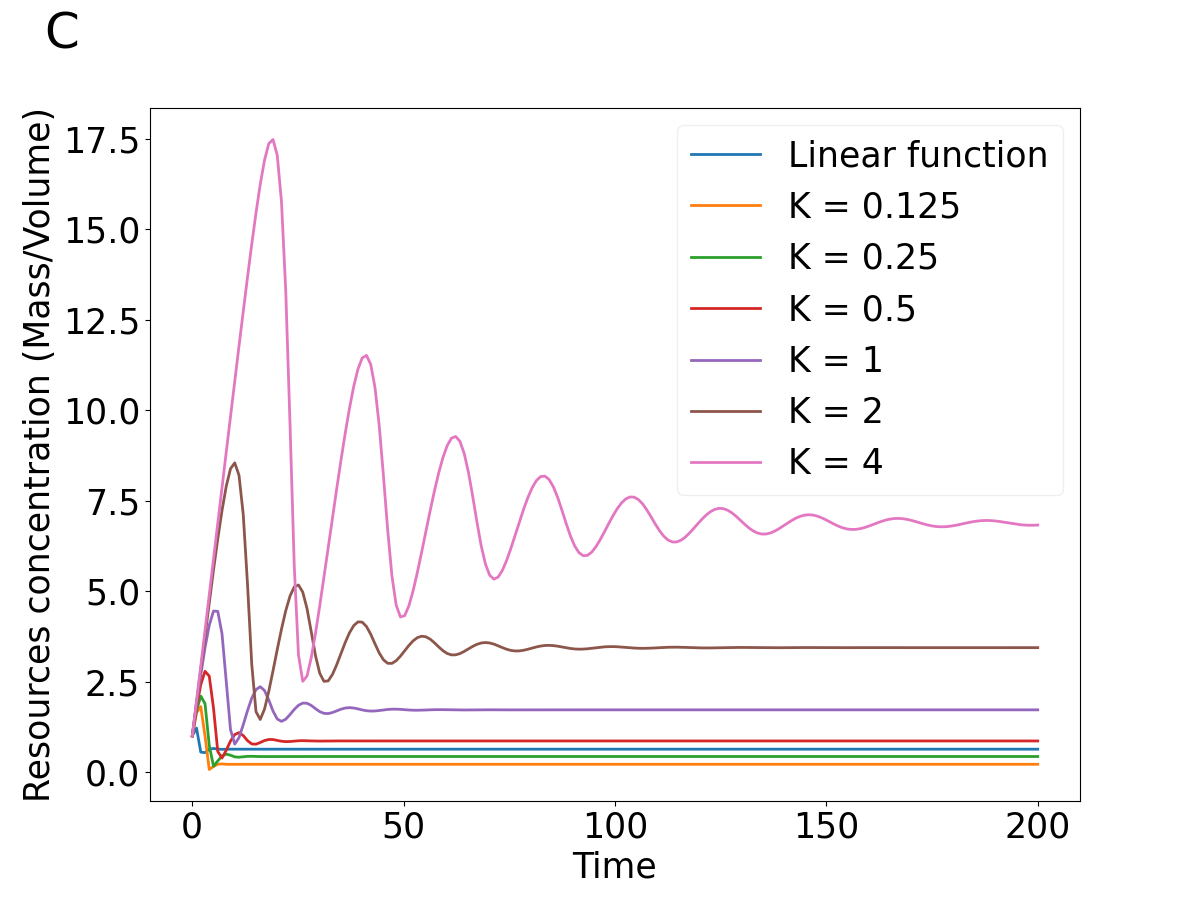
\includegraphics[scale=0.27]{./Figures/K_res.png}
    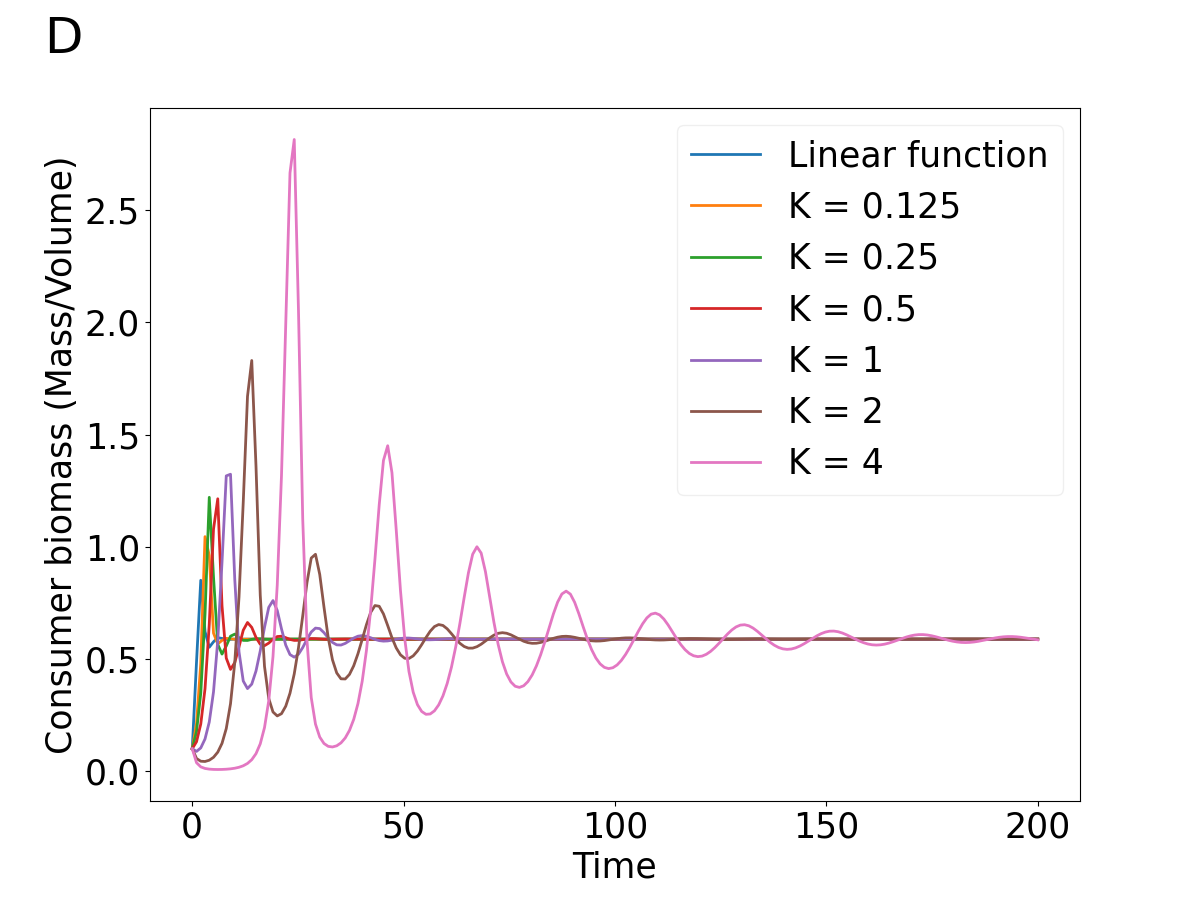
\includegraphics[scale=0.27]{./Figures/K_con.png}
    \end{tabular}
    \caption{\textbf{The temperature response of species richness with Type II functional response (Monod function) contained in species resource uptake.} A: The species uptake rates as a function of substrate resource concentration, $K$ denotes the half saturation constant. B: The temperature response of species richness with different K values. This plot shows that substituting linear functional response by Type II function response with different half saturation constants does not significantly impact species richness pattern with temperature. C \& D: The example of resource and consumer concentration dynamics of a single species with different half saturation constants in Monod function. }
    \label{fig:TypeII}
\end{figure}

\subsection{Interspeices interaction in high leakage environment}\label{sec:lf}

Here I show that changing leakage fractions does not significantly impact the temperature response pattern of species richness, with the exception of the highest leakage fraction of $l = 0.7$ (Figure \ref{fig:lf}A). And that that facilitation is favored at low temperatures for high leakage communities, at high temperatures for low leakage communities (Figure \ref{fig:lf}B). In Figure \ref{fig:lf}C, I demonstrate the interspecies interactions for communities with the extremely high leakage fraction of 0.7, it shows a sharper decrease of survivor resource overlap, and outweighing the increase of survivor facilitation at a lower temperature. Species with much higher resources partitions succeed competition (Figure \ref{fig:lf}D). Generally speaking, facilitation appears to be relatively unfavorable for communities at this leakage level. This indicates that facilitation is only beneficial for community coexistence to an extent, beyond that, the advantage of facilitative environment is outweighed by the detriments including the high resource leakage, and the extreme selection on species with lower resource overlap.

\begin{figure}
    \centering
    \begin{tabular}{c@{}c@{}}
    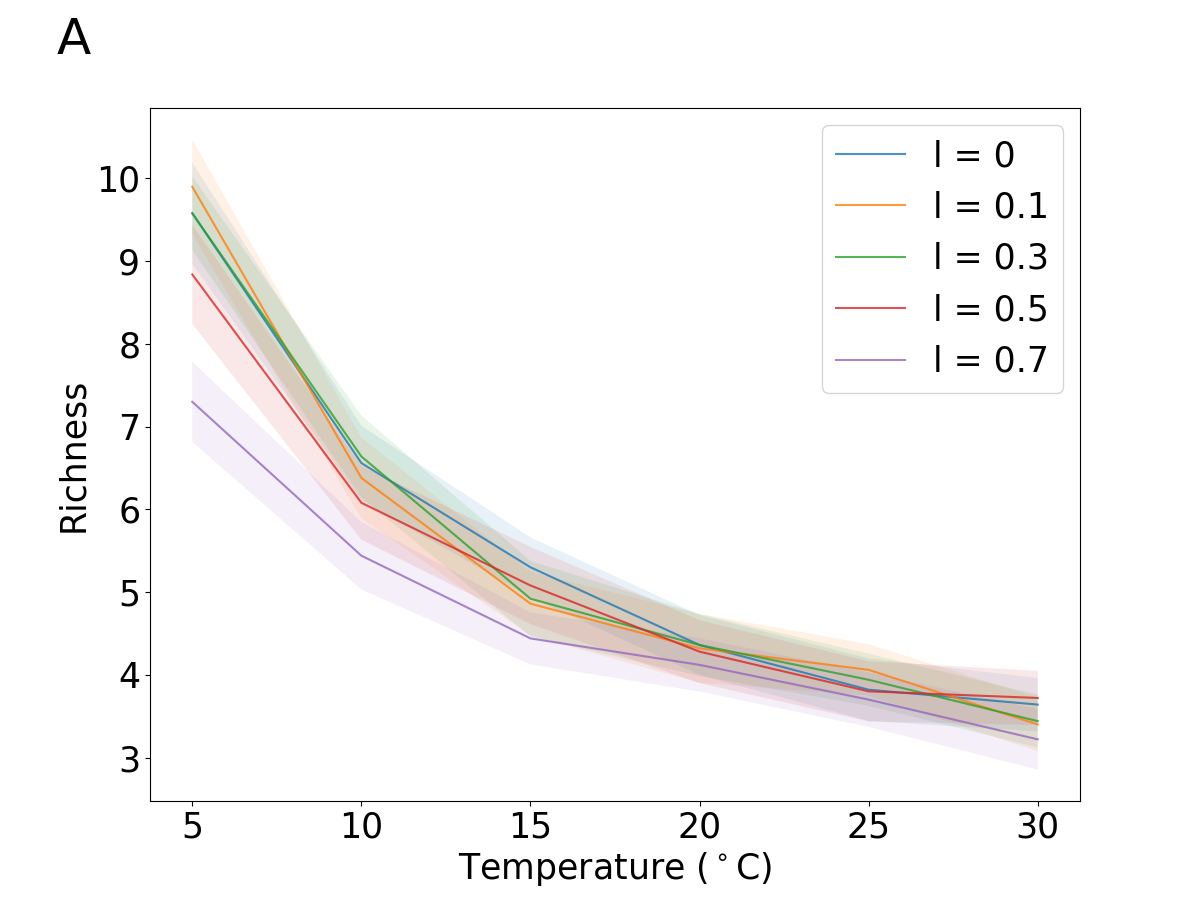
\includegraphics[scale=0.27]{./Figures/leakage_rich.png}
    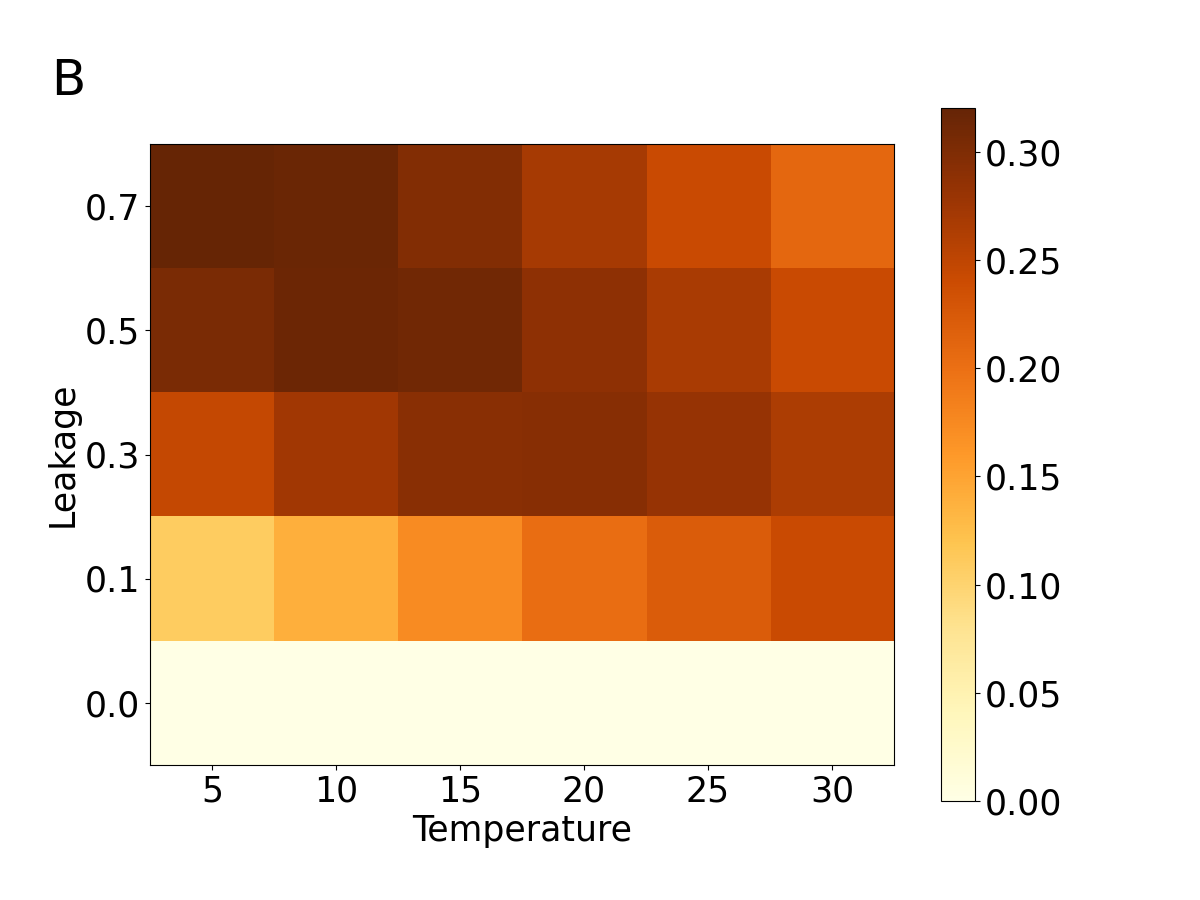
\includegraphics[scale=0.27]{./Figures/cf_lf.png}
    \end{tabular}
    \hfill\\
    \begin{tabular}{c@{}c@{}}
    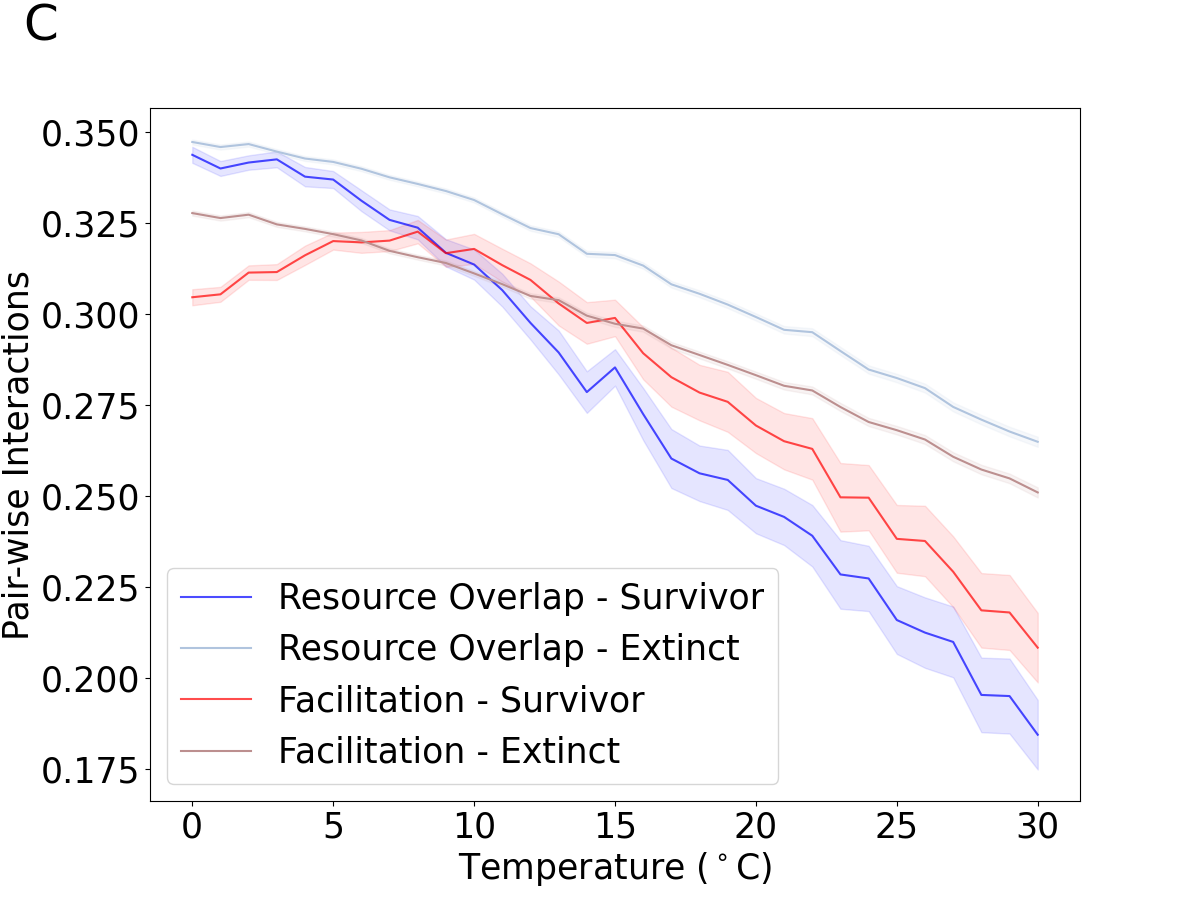
\includegraphics[scale=0.27]{./Figures/07.png}
    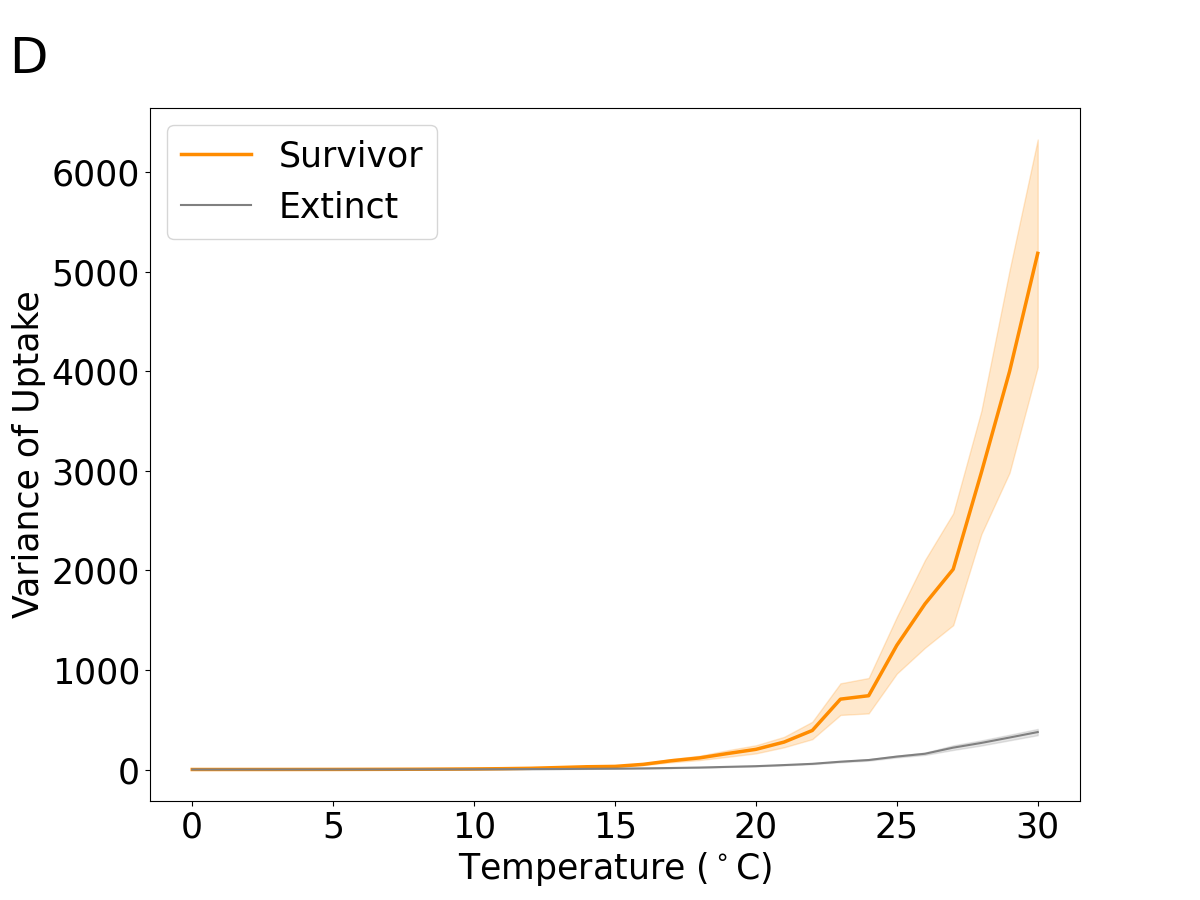
\includegraphics[scale=0.27]{./Figures/07_U.png}
    \end{tabular}
    \caption{\textbf{The relation between temperature dependent species richness pattern and the selection on interspecies facilitation.} Species richness at temperatures within OTR (A, plotted with 95\% CI bands for community richness values with each leakage fraction at each temperature) and the facilitation ability of survivors (B) at different leakage fraction and different temperatures. C and D demonstrates the resulting species interactions (C), and the variance of resources uptake (D) at different temperatures when setting leakage fraction to 0.7, with 95\% CI bands for these values in communities assembled at each temperature. (CI = 95\%)} 
    \label{fig:lf}
\end{figure}


\end{document}


\end{spacing}
\end{document}
